\documentclass[parskip=full,11pt,twoside]{scrartcl}
\usepackage[utf8]{inputenc}

\title{DCBN: Decision Critical Bayesian Networks}
\author{Johann Bonneau, Leo Garbe, Ruben Grewal, Fabio Mayer, Daniel Vollmer}

% section numbers in margins:
\renewcommand\sectionlinesformat[4]{\makebox[0pt][r]{#3}#4}

% header & footer
\usepackage{scrlayer-scrpage}
\lofoot{\today}
\refoot{\today}
\pagestyle{scrheadings}

\usepackage[sfdefault,light]{roboto}
\usepackage[T1]{fontenc}
\usepackage[german]{babel}
\usepackage[]{datetime} % must be after babel
\renewcommand{\dateseparator}{-} % ISO8601 date format
\usepackage{hyperref}
\usepackage{amsmath}
\usepackage[nameinlink]{cleveref}
\crefname{figure}{Abb}{Abb}
\usepackage[section]{placeins}
\usepackage{xcolor}
\usepackage{graphicx}
\usepackage[nonumberlist,toc,nopostdot]{glossaries}
\hypersetup{
	pdftitle={Pflichtenheft},
	bookmarks=true,
}
\usepackage{csquotes}

\usepackage{amsmath} % for $\text{}$
\newcommand\urlpart[2]{$\underbrace{\text{\texttt{#1}}}_{\text{#2}}$}

\usepackage{pflichtenheft}

\makeglossaries

\newglossaryentry{nutzer}{
name={Nutzer},
description={Ein Nutzer ist eine Person die das System benutzt.}
}
\newglossaryentry{moderator}{
name={Moderator},
description={Ein Moderator ist eine Person, dessen \Gls{konto} die wenigsten Rechte hat.}
}
\newglossaryentry{admin}{
name={Admin},
description={Ein Admin ist eine Person, dessen \Gls{konto} alle Funktionalitäten benutzen darf (außer die vom \Gls{superadmin}).}
}
\newglossaryentry{superadmin}{
name={Superadmin},
description={Ein Superadmin ist eine Person, die das ganze Benutzersystem verwalten kann.}
}
\newglossaryentry{evidenz}{
name={Evidenz},
description={Eine Evidenz ist in DCBN immer ein Wahrheitswert (true/false bzw 0/1) der den Wert eines Knotens angibt. Virtuelle Evidenzen können auch Werte zwischen 0 und 1 sein.}
}
\newglossaryentry{produktdaten}{
name={Produktdaten},
description={Die Daten, welche vom System persistiert werden.}
}
\newglossaryentry{gui}{
name={GUI},
description={Benutzeroberfläche (Graphical User Interface)}
}
\newglossaryentry{netz}{
name={Netz},
plural={Netze},
description={In DCBN immer ein dynamisches bayes'sches Netz (DBN).}
}
\newglossaryentry{knoten}{
name={Knoten},
plural={Knoten},
description={Ein Knoten eines \Gls{netz}es.}
}
\newglossaryentry{pfeil}{
name={Pfeil},
description={Ein Pfeil, der zwei \Gls{knoten} miteinander verbindet.}
}
\newglossaryentry{inferenz}{
name={Inferenz},
description={Der Prozess des Ausrechnens bzw. Evaluierens der DBNs. Also das Schließen von bekannten auf noch unbekannte Knoten-Werte.}
}
\newglossaryentry{IOSB}{
name={IOSB},
description={Fraunhofer-Institut für Optronik, Systemtechnik und Bildauswertung.}
}
\newglossaryentry{konto}{
name={Konto},
plural={Konten},
description={Repräsentiert die Zugriffsrechte und weite Informationen einer Person im System. Eine Person mit einen einem Konto kann sich mit Email und Passwort des Kontos im System einloggen.}
}
\newglossaryentry{zeitschritte}{
name={Zeitschritte},
description={Die Anzahl der Zeitschritte eines Netzes grenzt ein, über wie viele Schritte Zeitpfeile gehen können. Also auf wie viel Werte vorher man sich beziehen kann.}
}
\newglossaryentry{drag-and-drop}{
name={Drag-and-Drop},
description={Die Aktion von klicken, Klick halten, bewegen, Klick loslassen.}
}
\newglossaryentry{genie2}{
name={GeNIe2},
description={Ein Programm zur Erstellung und Auswertung von DBNs.}
}
\newglossaryentry{zeitpfeile}{
name={Zeitpfeil},
description={Pfeil, der eine zeitliche Abhängigkeit zwischen zwei \Glspl{knoten} anzeigt.}
}
\newglossaryentry{cache}{
name={Cache},
description={Caching bezeichnet das Zwischenspeichern von Daten. Meistens werden die Daten auf einem schnelleren Speichermedium gespeichert, um schnelleren Zugriff zu gewähren.  }
}
\newglossaryentry{modular}{
name={modular},
description={Ein System ist modular, wenn Veränderungen oder Ergänzungen an einer Stelle im System keinen zu großen Aufwand repräsentiert.}
}
\newglossaryentry{ActiveMQ}{
name={ActiveMQ},
description={Apache Active Message Queuing (ActiveMQ) ist eine Kommunikations-Schnittstelle, zwischen verschiedenen Systemen. }
}
\newglossaryentry{temporalplatte}{
name={Temporalplatte},
description={Das Konzept einer Temporalplatte ist hier eine Referenz zu einem Feature aus GeNIe.}
}


\begin{document}
\maketitle
\pagebreak
\tableofcontents

%\pagebreak

\section{Einleitung}

Eine kritische Situation ist eine Situation, die am Wendepunkt einer Krise analysiert wird. Um solche Situationen besser zu analysieren werden immer häufiger dynamische bayes'sche Netzwerke (DBN) benutzt. Was dafür jedoch noch fehlt, ist ein moderner und einfach zu bedienender Editor, um diese Netze zu erstellen. Unser Programm, Decision Critical Bayesian Networks (DCBN), soll diese Lücke schließen. Das Programm wird jedoch speziell für die Erkennung kritischer Situationen im maritimen Bereich, wie illegale Tauchgänge oder Menschen-Schmuggel, entwickelt. DCBN soll dem Nutzer erlauben die dynamischen bayes'sche Netze grafisch darzustellen und zu bearbeiten. Es bietet dem Benutzer über ein webbasiertes Graphical User Interface (GUI) die Möglichkeit ein neues Netz zu erstellen oder existierende Netze zu bearbeiten und zu testen. Nachdem ein solches Netz erstellt wurde, soll man die Inferenzen berechnen können, um die Situation besser zu analysieren. 
Unser Programm ist somit in zwei Teile aufgeteilt:
\begin{enumerate}
    \item \textbf{Frontend:} GUI zur Erzeugung, Darstellung und Testen der Netze.
    \item \textbf{Backend:} Server zum Speichern der Netze und zur Berechnung der Inferenzen. 
    
\end{enumerate}
\section{Kriterien}
% Diese Section sollte kurz und knapp "für Manager" sein
% und auf eine Seite passen.

\subsection{Muss}

%net zu netman geändert, evimake hinzugefügt
%Paar Dinge umsortiert. 
\criterium{Superadmin}{crt:sudo}
\criterium{Benutzersystem}{crt:usersys}
\criterium{Unterstützung für mehrere Sprachen}{crt:multiling}
\criterium{Ordnerstruktur für \Glspl{netz}}{crt:ordstr}
\criterium{Netze verwalten}{crt:netman}
\criterium{Netze erstellen/bearbeiten}{crt:netmake}
\criterium{Netze importieren}{crt:netimport} % Sollten die beiden nicht einfach zum Punkt "Netze verwalten" hinzugefügt werden?
\criterium{Netze exportieren}{crt:expo}
\criterium{Evidenzen verwalten}{crt:eviman}
\criterium{Evidenzen erstellen/bearbeiten}{crt:evimake}
\criterium{Testumgebung für Netze}{crt:playgr}
\criterium{\gls{inferenz} berechnen}{crt:infcal}
\criterium{Integration mit \gls{IOSB} Servern}{crt:IOSB}

\subsection{Kann}

%\criteriumOptional{Submodels in Netzen}{crt:submodplus}
\criteriumOptional{Netz-Kanten über mehr als einen Zeitschritt}{crt:tplus}
\criteriumOptional{Beispieldaten in der Testumgebung für Netze speichern/laden}{crt:playdataplus}
\criteriumOptional{Automatische Anordnung von Netzen}{crt:autolayoutplus}
\criteriumOptional{Live Daten-Stream in die Testumgebung für Netze}{crt:liveplus}
\criteriumOptional{Annotationsdaten Auswertung in Evidenzen}{crt:annotplus}

\subsection{Abgrenzung}

\criteriumNot{Temporal Unterscheidung}{crt:tempabgr}
Es gibt keine Unterscheidung welche \Gls{knoten} auf einer \Gls{temporalplatte} sind und welche nicht. Es wird angenommen, dass alle Knoten auf der \Gls{temporalplatte} sind und standardmäßig die Wahrscheinlichkeiten für t=0 modelliert werden.
\criteriumNot{Verschiedenen Knoten-Typen im Netz}{crt:typeabgr}
Es gibt lediglich normale Wahrscheinlichkeits-Knoten.
\criteriumNot{Unroll}{crt:unrollabgr}
Ein temporales Netz muss nicht automatisch zu einem nicht-temporalen Netz ausgerollt werden können.


%%%%%%%%%%%%%%
\section{Produkteinsatz}

Das Produkt soll mit minimalen Administrationskenntnissen zu betreiben sein.

Nutzer des Dienstes sollen diesen ohne Schulung oder andere Information benutzen können.

\section{Produktumgebung}

\textbf{Frontend:} Das Programm soll auf jedem modernen Webbrowser (IE 11+ und Safari 9+) laufen. Dazu sollen ca. 4GB RAM zur Verfügung stehen (abhängig vom Webbrowser).

% IST DAS WIRKLICH SINNVOLL HIER EXPLIZIT DIE KERNE ZU ERWÄHNEN? IM GESPRÄCH HAT ER GEMEINT, DASS WIR UNS DAS ÜBERLEGEN SOLLEN!!!!
\textbf{Backend:} Server mit mindestens 4 Kernen und mindestens 8GB DDR3+ RAM.

\section{Nutzerrechte}

\subsection{Alle Nutzer}
Alle \Gls{nutzer} sind in der Lage die Sprache zu ändern und sich an- bzw. abzumelden.

% fnc:changeLang, fnc:logoutAll

\subsection{Moderator}
Ein \Gls{moderator} hat zusätzlich das Recht, die Testumgebung für Netze zu nutzen und Netze zu exportieren. % Ist jetzt halt schon scheiße, wenn da keine Links zu den FAs sind.

% fnc:play, fnc:expnet.

\subsection{Admin}
Ein \Gls{admin} hat zusätzlich zu den Moderatorrechten die Rechte, den Netzeditor zu nutzen, die Ordnerstruktur zu verändern (Ordner/Netze umbenennen, duplizieren, usw.), sowie Netze zu importieren.

% Links für die FAs...

\subsection{Superadmin}
Der \Gls{superadmin} verfügt lediglich über das Recht der \Gls{konto}verwaltung.
% LINKS

%%%%%%%%%%%
\section{Funktionale Anforderungen}

\subsection{Benutzersystem}
\subsubsection{Superadmin}

\functionality{Festes Superadmin-\Gls{konto}}{fnc:sudoinit}
\fulfills{crt:sudo}
Das Programm soll mit einem festgelegten Superadmin-Nutzer initialisiert werden. Die Logindaten des \Gls{superadmin}s werden dem Kunden mitgeteilt.

\functionality{Nach Konten suchen}{fnc:searchusr}
\fulfills{crt:sudo}
Der \Gls{superadmin} soll in der Lage sein, nach existierenden \Glspl{konto} zu suchen. Diese Suche erfolgt über Name, Benutzername, Rolle oder Email-Adresse des gesuchten Nutzers. Dabei wird immer eine Liste an Nutzern angezeigt, die der Suchanfrage in irgendeiner Form entsprechen.

\functionality{Konten erstellen}{fnc:addusr}
\fulfills{crt:sudo}
\fulfills{crt:usersys}
Der Superadmin kann neue Konten erstellen. Dafür muss der Superadmin Benutzername, Name, Email und Rolle des Nutzers beim Erstellen eingeben.


\functionality{Konten löschen}{fnc:delusr}
\fulfills{crt:sudo}
\fulfills{crt:usersys}
Der Superadmin kann Nutzer (Admins und Moderatoren) löschen. 

\functionality{\Gls{konto}daten ändern}{fnc:editusr}
\fulfills{crt:sudo}
\fulfills{crt:usersys}
Der Superadmin kann Nutzerdaten wie Name, Email, Benutzername oder Rolle eines Nutzers ändern.

\subsubsection{Startseite}

% Bei der Definition des Kontos steht dass der Nutzer sich mit Email anmeldet. Eins davon sollte man anpassen.
\functionality{Anmelden}{fnc:login}
\fulfills{crt:usersys}
Auf der Startseite soll man sich mit Benutzername und Passwort anmelden können.


\functionality{Passwort-Zurücksetzung anfordern}{fnc:resetpass}
\fulfills{crt:usersys}
Falls man sein Passwort vergessen hat, kann man anfordern, dass das Passwort zurückgesetzt wird. Man erhält dann eine Email mit einem Link zur Passwort-Wiederherstellung.  

\functionality{Neues Passwort festlegen}{fnc:editpass}
\fulfills{crt:usersys}
Der Nutzer soll mit dem Link in der Email ein neues Passwort festlegen können. Danach kann der Nutzer sich mit dem neuen Passwort anmelden.

% \functionality{Abmelden}{fnc:logout}
% \fulfills{crt:usersys}
% Der Moderator soll sich abmelden können und wieder auf der Login-Seite landen. 

\subsection{Grundlegendes}

\functionality{Abmelden}{fnc:logoutAll}
\fulfills{crt:usersys}
Jeder Nutzer hat die Möglichkeit, sich durch einen Klick auf den \enquote{Logout}-Knopf abzumelden. Dabei gelangt er zurück zur Anmelde-Seite und wird beim Neuladen der Seite nicht mehr automatisch angemeldet.

\functionality{Sprache ändern}{fnc:changeLang}
\fulfills{crt:multiling}
Im Menü wird dem Nutzer die aktuell ausgewählte Sprache angezeigt (standardmäßig Englisch). Durch einen Klick auf diese öffnet sich ein Drop-Down-Menü in dem der Nutzer eine andere Sprache auswählen kann. Tut der Nutzer dies, ändern sich automatisch alle Texte auf die entsprechende Sprache.

\subsection{Netzverwaltung}  

\functionality{Netze importieren}{fnc:netimport}
\fulfills{crt:netimport}

Ein Administrator ist in der Lage Netze zu importieren. Dies bedeutet, dass lokal gespeicherte Netze auf den Server hochgeladen werden. Hierbei muss die Datei eines der folgenden Formate haben:
\begin{enumerate}
    \item .xdsl - \gls{genie2} Format
    \item .net - Hugin Format % Stimmt das überhaupt? 
    % Noch andere
    
\end{enumerate}
\functionality{Netze exportieren}{fnc:expnet}
\fulfills{crt:expo}
Ein Moderator ist in der Lage ein Netz zu exportieren. Dies bedeutet, dass der Moderator Netze, die auf dem Server gespeichert sind, herunterladen kann. Hierbei kann der Moderator eines der folgenden Formate zum Exportieren auswählen:
\begin{enumerate}
    \item .xdsl - GeNIe2 Format
    \item .net - Hugin Format % Stimmt das überhaupt? 
\end{enumerate}

\functionality{Netze umbenennen}{fnc:renamenet}
\fulfills{crt:netman}
Ein Administrator ist in der Lage Netze umzubenennen. Hierzu klickt er mit der rechten Maustaste auf das Netz im Dateibaum und wählt im Rechtsklickmenü die Option \enquote{Rename}. In dem sich öffnenden Fenster gibt der Nutzer den neuen Namen des Netzes ein und bestätigt den Namen mit der \enquote{Enter}-Taste oder durch einen Klick auf den \enquote{Confirm}-Knopf. Sollte der eingegebene Name ungültig sein (Netz mit selbem Namen existiert bereits in diesem Ordner, ungültige Zeichen, usw.), so wird eine Fehlermeldung ausgegeben und der Name wird nicht übernommen.

\functionality{Netze duplizieren}{fnc:copynet}
\fulfills{crt:netman}
% Ist das Kopieren nur ein Duplizieren in den selben Ordner oder ein Copy-Paste auch in andere Ordner?
% Falls Letzteres, bräuchte man dann nicht auch noch eine FA zum Einfügen?

%(Ruben)Ich glaube es ist nur als eine Kopie von Netz im selben Ordner erstellen gedacht (Copy of Net.xddsl)

Ein Administrator ist in der Lage Netze durch ein Tastenkürzel bzw. ein Rechtsklickmenü Netze zu kopieren. Dabei wird das komplette Netz in den selben Ordner dupliziert.

\functionality{Netze löschen}{fnc:delNet}
\fulfills{crt:ordstr}
\fulfills{crt:netman}

Durch einen Rechtsklick auf ein Netz öffnet sich ein Drop-Down-Menü mit der Option \enquote{Delete}. Wird diese ausgewählt, so öffnet sich ein Dialog mit einer Warnung in der das Löschen erneut bestätigt werden muss. Wird dies getan, so wird das Netz entfernt.
Falls das Netz aktuell bearbeitet wird, schlägt die Aktion fehl und eine Fehlermeldung wird angezeigt.

\subsection{Ordnerstruktur}

\functionality{Netze in Ordner schieben}{fnc:putNetInFol}
\fulfills{crt:ordstr}
\fulfills{crt:netman}

Durch einen Rechtsklick auf ein Netz öffnet sich ein Drop-Down-Menü mit der Option \enquote{Move}.
Wird diese ausgewählt, so öffnet sich ein Dialog mit einem Abbild der Ordnerstruktur in der der aktuelle Ordner ausgewählt ist. Hier kann ein anderer ausgewählt werden und durch ein Klick auf \enquote{Confirm} die Änderung wirksam gemacht werden.
Falls das Netz aktuell bearbeitet wird, schlägt die Aktion fehl und eine Fehlermeldung wird angezeigt.

\functionality{Ordner umbenennen}{fnc:modFolName}
\fulfills{crt:ordstr}

Durch einen Rechtsklick auf einen Ordner öffnet sich ein Rechtsklickmenü mit der Option \enquote{Rename}. Wird diese ausgewählt, so öffnet sich ein Dialog mit einem Eingabefeld, in dem der aktuelle Name des Ordners steht. Hier kann dieser geändert werden und durch ein Klick auf \enquote{Confirm} die Änderung wirksam gemacht werden.
Falls ein DBN in dem ausgewählten Ordner aktuell bearbeitet wird, schlägt die Aktion fehl und eine Fehlermeldung wird angezeigt.

\functionality{Ordner löschen}{fnc:delFol}
\fulfills{crt:ordstr}

Durch einen Rechtsklick auf einen Ordner öffnet sich ein Rechtsklickmenü mit der Option \enquote{Delete}. Wird diese ausgewählt, so öffnet sich ein Dialog mit einer Warnung in der das Löschen erneut bestätigt werden muss. Wird dies getan, so wird der Ordner mit allen Unterordnern und DBNs entfernt.
Falls ein DBN in dem ausgewählten Ordner aktuell bearbeitet wird, schlägt die Aktion fehl und eine Fehlermeldung wird angezeigt.


% Rechtsklickmenü eigene FA?
\subsection{Netz-Editor}

\functionality{Netze öffnen}{fnc:opennet}
\fulfills{crt:netmake}
\fulfills{crt:netman}
Im Netzeditor kann ein Netz durch einen Klick auf den Dateinamen des Netzes im Dateibaum geöffnet werden. Dieses muss auf dem Server liegen.

\functionality{Netze erstellen}{fnc:makenet}
\fulfills{crt:netmake}
Im Netzeditor kann ein neues Netz durch einen Klick auf den \enquote{Create Net}-Knopf im Dateibaum erstellt werden. Hierfür wird ein neues, leeres und temporäres Netz erstellt. Diesem kann man durch Speichern des Netzes einen festen Speicherort in der Ordnerstruktur zuweisen.

\functionality{Netz speichern}{fnc:savenet}
\fulfills{crt:netman}
% Vielleicht anders formulieren falls ihr immer noch verwirrt seid.
Im Netzeditor kann ein Netz durch das als Standard angesehene Tastenkürzel des jeweiligen Betriebssystems zum Speichern bzw. durch einen Klick auf den \enquote{Save}-Knopf (siehe \Cref{section:gui}) gespeichert werden.

\functionality{Netz sperren wenn Netz bearbeitet wird}{fnc:locknet}
\fulfills{crt:netman}
Jeweils nur ein Admin kann ein Netz zur selben Zeit bearbeiten. Sollte ein Netz bereits von einem Admin bearbeitet werden, so wird bei dem Versuch eines anderen Admins auf das Netz zuzugreifen eine Fehlermeldung zurückgegeben.

% TODO: Vielleicht Teil der Ordnerstruktur?
\functionality{Zeitschritte vom Netz einstellen}{fnc:settempsteps}
\fulfills{crt:netmake}
Im Netzeditor kann die Anzahl an \gls{zeitschritte}n des Netzes eingestellt werden. Hierfür ändert der Nutzer den Wert im Eingabefeld bei \enquote{Timesteps}. Dieser Wert lässt sich nur auf valide Werte ändern. Hat das Netz beispielsweise einen 2er Zeitpfeil, so wäre \enquote{1} kein legitimer Wert und die Eingabe nicht möglich. Des Weiteren kann der Wert 100 nicht überschritten werden. 

\functionality{Knoten hinzufügen}{fnc:addnode}
\fulfills{crt:netmake}
Im Netzeditor kann ein neuer Knoten zu einem Netz hinzugefügt werden. Hierfür wählt der Nutzer den \enquote{Add Node}-Knopf aus und klickt auf das Bearbeitungsfenster der Editor-GUI. Ein komplett leerer Knoten wird an der angeklickten Stelle erzeugt.
Der Knoten hat zwei Zustände (\enquote{true} und \enquote{false}) welche beide eine Wahrscheinlichkeit von 0.5 haben.


% Sollte der Nutzer vielleicht noch vorher gefragt werden, ob er den Knoten wirklich löschen will?
\functionality{Knoten löschen}{fnc:delnode}
\fulfills{crt:netmake}
Wählt der Nutzer einen Knoten aus, so kann er diesen Knoten durch Betätigen der \enquote{Delete}-Taste bzw. durch einen Klick auf \enquote{Delete} im Rechtsklickmenü aus dem Netz entfernen. Sollte der gelöschte Knoten durch \gls{pfeil}e mit anderen Knoten verbunden sein, so werden alle mit diesem Knoten verbundenen Pfeile automatisch auch gelöscht.

\functionality{Knoten bewegen}{fnc:movenode}
\fulfills{crt:netmake}
Der Nutzer kann beliebige Knoten durch \gls{drag-and-drop} innerhalb des selben Netzes verschieben. Hierbei werden mögliche Verbindungen zwischen den Knoten automatisch angepasst. Sollte der verschobene Knoten einen anderen Knoten überdecken, so wird die Verschiebung nicht ausgeführt.

\functionality{Knoten Name ändern}{fnc:renamenode}
\fulfills{crt:netmake}
Ein Knoten kann durch einen Klick auf \enquote{Rename} im Rechtsklickmenü oder mit einem Doppelklick auf den Namen des Knoten umbenannt werden.

% Vielleicht sollte man für dieses Eigenschaften Menü eine eigene FA hinzufügen...
\functionality{Knoten Farbe ändern}{fnc:cngcolor}
\fulfills{crt:netmake}
Die Hintergrundfarbe eines Knoten kann im \enquote{Properties}-Menü des Knotens geändert werden. Hierfür macht der Nutzer einen Doppelklick auf den Knoten oder wählt \enquote{Properties} im Rechtsklickmenü des Knotens aus. Die Farbe des Textes des Knotens wird automatisch angepasst, um die Lesbarkeit des Textes zu gewährleisten. % Kann der Nutzer eine beliebige Farbe wählen, oder gibt es nur vorgewählte Möglichkeiten?
% Wie genau sieht das Eigenschaften Menü des Knoten aus, öffnet sich wie in GeNie ein eigenes Fenster, oder wird das Ganze im unteren Teil des Editors angezeigt?

\functionality{Wahrscheinlichkeiten eingeben}{fnc:insert}
\fulfills{crt:netmake}
Im \enquote{Properties}-Menü des Knoten kann der Nutzer die von der Inferenz verwendeten Wahrscheinlichkeiten angeben. Hierfür wird dem Nutzer eine Tabelle mit allen Kombinationsmöglichkeiten präsentiert, welche in den durch Pfeile vorangehenden Knoten-Ergebnissen auftreten können (vgl. mit GeNie2). Dem Nutzer wird außerdem die Möglichkeit gegeben, die bereits eingegebenen Wahrscheinlichkeiten einer Spalte zu \enquote{Eins} zu ergänzen. Gibt der Nutzer Wahrscheinlichkeiten ein, welche sich nicht zu \enquote{Eins} addieren, so werden beim Speichern die Wahrscheinlichkeiten ihrem Verhältnis entsprechend zu \enquote{Eins} angepasst. (D.h. Eingaben von 5 bei \enquote{true} und 2 bei \enquote{false} werden zu 0.714 und 0.286 geändert)

\functionality{Pfeile hinzufügen}{fnc:addarrow}
\fulfills{crt:netmake}
Im Netzeditor kann ein neuer Pfeil zu einem Netz hinzugefügt werden. Hierfür wählt der Nutzer den \enquote{Add Arrow} Knopf aus und klickt zuerst auf den Startknoten und dann auf den Endknoten im Bearbeitungsfenster. Daraufhin werden beide Knoten durch einen Pfeil verbunden. % Standardpfeil auf sich selbst in Zeitpfeil umwandeln oder einfach nicht zulassen?

\functionality{Zeitpfeile hinzufügen}{fnc:addtimearrow}
\fulfills{crt:netmake}
\fulfills{crt:tplus}

Im Netzeditor kann ein neuer Zeitpfeil zu einem Netz hinzugefügt werden. Hierfür wählt der Nutzer den \enquote{Add Time Arrow}-Knopf aus und klickt zuerst auf den Startknoten und dann auf den Endknoten im Bearbeitungsfenster. Daraufhin werden beide Knoten durch einen Zeitpfeil verbunden. Der Nutzer hat dann die Möglichkeit durch ein Eingabefeld die Anzahl der betrachteten Zeitschritte festzulegen. Diese Anzahl muss hierbei im Intervall zwischen 1 und 100 liegen (beide einschließlich). Die Bestätigung der Eingabe erfolgt durch Drücken der \enquote{Enter}-Taste oder durch Klicken außerhalb des Eingabefelds. Sollte der Nutzer eine ungültige Eingabe gemacht haben (keine Ganzzahl im verlangten Intervall), so wird die Anzahl der Zeitschritte automatisch auf 1 gesetzt.

\functionality{Pfeile löschen}{fnc:delarrow}
\fulfills{crt:netmake}
Wählt der Nutzer einen Pfeil aus, so kann er diesen Pfeil durch Betätigen der \enquote{Delete}-Taste bzw. durch einen Klick auf \enquote{Delete} im Rechtsklickmenü aus dem Netz entfernen. Die Wahrscheinlichkeitstabelle des Endknotens wird dementsprechend angepasst. Dies funktioniert sowohl für \gls{zeitpfeile}e als auch für normale Pfeile.

\functionality{\gls{evidenz} einem Knoten zuweisen}{fnc:assignevi}
\fulfills{crt:netmake}
\fulfills{crt:eviman}
Der Nutzer kann einem Knoten eine Evidenz zuweisen. Hierfür wählt er im \enquote{Properties}-Menü des Knotens den Reiter \enquote{Evidences} aus. Hier kann der Nutzer einem Knoten durch ein Drop-Down-Menü eine der bestehenden Evidenzen zuordnen. % Durch Druck auf den \enquote{Create Evidence}-Knopf öffnet sich der Evidenzeneditor??

% Was passiert wenn der Nutzer einfach nur den Zwischenstand speichern will und das Netz nicht valide ist.
% Wie wird das behandelt.
\functionality{Netz Validieren (DAG, Zusammenhängend)}{fnc:validatenet}
Beim Speichern des Netzes wird es validiert. Hierbei wird eine Warnung ausgegeben, falls das Netz nicht zusammenhängend ist und das falls es kein DAG ist, werden die Änderungen nicht übernommen.

% Letzte Schritte??? Vielleicht bis zu 20?
\functionality{Letzten Schritt rückgängig machen}{fnc:undo}
\fulfills{crt:netmake}
Durch einen Klick auf den \enquote{Undo}-Knopf oder durch das Tastenkürzel \enquote{CTRL + z} kann die zuletzt durchgeführte Aktion rückgängig gemacht werden. Dies kann für die letzten 20 Aktionen durchgeführt werden.

\functionality{Rückgängig gemachte Aktion wieder herstellen}{fnc:redo}
\fulfills{crt:netmake}
Durch einen Klick auf den \enquote{Redo}-Knopf oder durch das Tastenkürzel \enquote{CTRL + y} kann die zuletzt rückgängig gemachte Aktion wiederhergestellt werden. Es können nur so lange Aktionen wiederhergestellt werden, bis der Nutzer eine andere Aktion ausführt oder man wieder im Ursprungszustand angekommen ist.

%\functionality{Submodel erstellen}{fnc:createsubmodel}
%\fulfills{crt:netmake}
%\fulfills{crt:submodplus}
%Der Nutzer kann Submodelle definieren. Dies sind Netze, welche in anderen Netzen als Knoten eingefügt werden können.
% Man muss noch klären, was genau alles möglich ist. Kann man z.b. schon bestehende Netze zu Submodellen machen, wie wählt man Submodelle die man hinzufügen will aus, ...
% Es gibt derzeit auch noch keinen Test, da ich nicht genau weiß wie das in der GUI umgesetzt wird.

\functionality{Auto-Darstellung}{fnc:autolayoutplus}
\fulfills{crt:netmake}
\fulfills{crt:autolayoutplus}
Durch einen Klick auf den \enquote{Auto-Layout}-Knopf werden die Knoten und Pfeile des aktuellen Netzes dem zuletzt ausgewählten Algorithmus entsprechend angeordnet. Anhand eines Pfeil-Drop-Down-Menüs an der rechten Seite des \enquote{Auto-Layout}-Knopfes kann man den Algorithmus auswählen, welcher verwendet werden soll.

\subsection{Evidenz-Editor}

\functionality{Evidenzen erstellen}{fnc:creaEvi}
\fulfills{crt:evimake}

Durch einen Klick auf den \enquote{New Evidence}-Knopf öffnet sich der Evidenz-Editor. 
Der Benutzer kann den Namen der Evidenz oben in einem Eingabefeld eingeben.
Die Evidenzen werden in Form von logischen Formeln dargestellt. Diese werden in ein Eingabefeld eingegeben.
Durch einen Klick auf den \enquote{Save}-Knopf wird die erstellte Evidenz mit dem angegebenen Namen gespeichert.
Falls kein Name, keine Formel oder eine falsche Formel (z.B falsche Klammerung)... eingegeben wurde, scheitert das Speichern und eine Fehlermeldung wird angezeigt.

\functionality{Information Seite}{fnc:showInfo}

Durch einen Klick auf den \enquote{Info}-Knopf wird eine Pop-Up-Seite angezeigt.
Auf dieser werden allgemeine Informationen zu Evidenz-Formeln angezeigt, sowie auch eine Liste aller verfügbaren Operatoren und Methoden.
Durch einen Klick auf den \enquote{Close}-Knopf wird die Pop-Up-Seite geschlossen.

\functionality{Formel eingeben}{fnc:entForm}
\fulfills{crt:evimake}

Der Benutzer kann eine Aussagenlogische Formel im Formel-Eingabefeld eingeben.
Diese Verknüpfungen stehen zur Verfügung : \{=, >, >=, <, <=, !, \&, |\}.
Des Weiteren kann der Benutzer vordefinierte Methoden nutzen (in den Informationen beschrieben).
Der Benutzer kann auch Variablen eingeben. Diese Variablen stehen dann zum Testen zur Verfügung.

\functionality{Evidenzen bearbeiten}{fnc:modEvi}
\fulfills{crt:evimake}

Durch einen Klick auf den \enquote{Edit}-Knopf (mit einen Bleistift dargestellt)
wird die ausgewählte Evidenz im Editor angezeigt. Der Benutzer kann sie dann bearbeiten und testen.

\functionality{Formeln mit Beispieldaten testen}{fnc:testCalc}

Der Benutzer kann eine Formel, testen die er bereits eingegeben hat. Dazu muss er seine Variablen in der Liste suchen und den Wert eingeben. Durch Klick auf den \enquote{Test}-Knopf wird das Ergebnis angezeigt (false/true).

\functionality{Vordefinierte Funktionen in Formeln nutzen}{fnc:callFnc}

Es gibt vordefiniert Funktionen, die der Benutzer in die Formeln einsetzen kann. Die Liste und Beschreibung der Funktionen steht in der Information Pop-Up-Seite.

\functionality{Evidenzen löschen}{fnc:delEvi}

Durch einen Klick auf den \enquote{Delete}-Knopf (durch einen Mülleimer dargestellt) wird die ausgewählte Evidenz gelöscht. Es wird durch ein Pop-Up-Fenster nachgefragt ob der Benutzer diese Aktion wirklich durchführen möchte.
Durch einen Klick auf den \enquote{Yes}-Knopf wird die Evidenz gelöscht und das Pop-Up-Fenster geschlossen.
Durch einen Klick auf den \enquote{No}-Knopf wird die Evidenz nicht gelöscht und das Pop-Up-Fenster geschlossen.

\subsection{Testumgebung für Netze}

\functionality{Netz graphisch anzeigen}{fnc:showgraph}
\fulfills{crt:playgr}

Durch einen Klick auf ein Netz in der Ordner Ansicht wird das Netz angezeigt. 
Der Benutzer kann in der graphischen Ansicht das Netz, aber nicht die Knoten bewegen.

\functionality{Virtuelle Evidenzen einsetzen}{fnc:setVirEvi}
\fulfills{crt:playgr}

Durch Doppelklick auf einen Knoten taucht ein Pop-Up-Fenster auf, in dem der Benutzer eine virtuelle Evidenz eingeben kann.
Dem Benutzer liegen 2 Eingabefelder vor. Ein  \enquote{true} Feld und ein \enquote{false} Feld. In den Feldern können Werte zwischen 0 und 1
eingegeben werden.
Die Summe der Werte muss gleich 1 sein.
Virtuelle Evidenzen überschreiben bereits existierende Werte.

\functionality{Virtuelle Evidenzen löschen}{fnc:delVirEvi}
\fulfills{crt:playgr}

Durch Doppelklick auf einen Knoten erscheint ein Pop-Up-Fenster, in dem der Benutzer eine virtuelle Evidenz eingeben kann.
Er kann auf den \enquote{Remove}-Knopf Klicken, um die Evidenz zu löschen.
Falls schon Berechnungen durchgeführt wurden und eine Evidenz eingegeben wurde, werden die Berechnungen automatisch neu durchgeführt.

\functionality{Alle Virtuelle-Evidenzen löschen}{fnc:delAllVirEvi}
\fulfills{crt:playgr}

Der Nutzer kann durch einen Klick auf \enquote{Clear Graph}, alle im Netz eingetragenen virtuellen Evidenzen entfernen. Dabei werden auch alle Diagramme zurückgesetzt, die mögliche Inferenz-Ergebnisse anzeigen.

\functionality{Evidenzen/Berechnungen graphisch anzeigen}{fnc:showVirEvi}
\fulfills{crt:playgr}

Nachdem eine Berechnung durchgeführt wurde, werden die Ergebnisse im Knoten durch ein horizontales Stab-Diagramm angezeigt.

\functionality{Aktueller Stand des Graphen speichern}{fnc:saveGraphState}
\fulfills{crt:playdataplus}

Nachdem der Benutzer den Graphen ausprobiert hat, hat er die Möglichkeit seinen Test zu speichern.
Durch Klick auf den \enquote{Export State}-Knopf wird ein Pop-Up-Fenster angezeigt. Dort kann der Nutzer einen Namen für den Test angeben.
Durch einen Klick auf den \enquote{Save}-Knopf wird der Name überprüft und dann der Test gespeichert.
Durch einen Klick auf den \enquote{Cancel}-Knopf wird der Speichervorgang abgebrochen.
Der Zustand wird in einer \enquote{.json} Datei gespeichert. Die Datei wird dann vom Browser heruntergeladen.

%%%%%%%%%%%%%%%%%%%Import State Knoipf fehlt?%%%%%%%%%%%%%%%%%%%%%

\functionality{Stand eines Graphen benutzen}{fnc:loadGraphState}
\fulfills{crt:playdataplus}

Der Benutzer kann den Stand eines Graphen benutzen. Beim Laden des Standes werden die Werte eingesetzt und automatisch die Berechnungen durchgeführt.

\functionality{Daten-Stream auswählen}{fnc:loadDataStream}
\fulfills{crt:liveplus}

Der Benutzer kann einen zur Verfügung gestellten Daten-Stream zur Ausführung auswählen.

\subsection{Server}

%\functionality{ REST-Schnittstelle für Frontend }{fnc:interface}

\functionality{ Daten von IOSB-Servern empfangen }{fnc:getServData}
Sobald Daten in der \gls{ActiveMQ} der IOSB-Server anliegen werden diese entsprechend deserialisiert und für die Inferenz bereitgestellt.
\fulfills{crt:IOSB}

\functionality{ Nötige Daten \gls{cache}n }{fnc:cacheData}
Für die Inferenz eines DBNs mit N Zeitschritten, werden insbesondere die Datensätze für die letzten N Zeitintervalle benötigt. Der Server stellt also sicher, dass immer zumindest der jeweils letzte Datensatz aus den M vorherigen Zeitintervallen zur Verfügung steht. Wobei M die größte Anzahl an Zeitschritten aller DBNs ist.
\fulfills{crt:IOSB}

\functionality{ Evidenz-Formeln interpretieren }{fnc:intInf}
Die Evidenz-Formeln beschreiben eine Verknüpfung der DBN-Knoten mit gegebenen Datensätzen. Diese Formeln müssen zum Zeitpunkt der Inferenz vom Server für gegebene Daten interpretiert und evaluiert werden.
\fulfills{crt:IOSB}
\fulfills{crt:infcal}

\functionality{ Evidenz-Formeln für Annotationen }{fnc:infAnnot}
Es besteht die Möglichkeit, dass Evidenz-Formeln nicht nur für gegebene Datentypen evaluiert werden können, sondern auch für beliebige Annotationen.
\fulfills{crt:annotplus}

\functionality{ Inferenz berechnen }{fnc:calcInf}
Für ein DBN kann der Server mit Hilfe einer Inferenz-Engine die Inferenz berechnen. Hierzu können entweder virtuelle Evidenzen aus der Testumgebung für Netze vorliegen oder die tatsächlichen Datensätze von den IOSB-Servern.
\fulfills{crt:IOSB}
\fulfills{crt:infcal}

\functionality{ Inferenz-Ergebnisse an IOSB Server senden }{fnc:sendRes}
Die Ergebnisse der Inferenz für gegebene Datensätze werden in Echtzeit an die IOSB-Server zur weiteren Verarbeitung zurückgegeben. Hierbei müssen die Ergebnisse in ein von den IOSB-Servern akzeptiertes Format serialisiert werden.
\fulfills{crt:IOSB}

%%%%%%%%%%%%%%%%%%%%%%%%%%%%%
\section{Produktdaten}
Die Persistierung der jeweiligen \Gls{produktdaten} erfolgt in einer beliebigen Datenbank, die Object Mapping von Spring Boot unterstützt.

\prodData{Benutzer}
Die folgenden Daten werden für Nutzer-Konten gespeichert:
\begin{itemize}
  \item Name
  \item Nutzername
  \item Email Adresse
  \item Rolle
  \item Hash des Passworts
\end{itemize}

\prodData{Netze}
Die folgenden Daten werden für Netze gespeichert:
\begin{itemize}
  \item Name
  \item Virtueller Ordner-Pfad
  \item Zeitschritte
  \item Graphstruktur
\end{itemize}

\prodData{Evidenz-Formeln}
Die folgenden Daten werden für Evidenz-Formeln gespeichert:
\begin{itemize}
  \item Name
  \item Formel-Ausdruck (keine Semantik)
\end{itemize}

\section{Nicht-Funktionale Anforderungen}

\nonFunctionality{Moderne \gls{gui}}{nfc:GUI}

%Material Design erwähnen.
Die GUI soll modern und einfach zu nutzen sein. Dazu werden grundlegende Material Design Guidelines eingehalten.

\nonFunctionality{50 gleichzeitige Nutzer}{nfc:concurrent}

Es sollen 50 \Gls{nutzer} gleichzeitig an verschiedenen Netzen arbeiten dürfen. 

\nonFunctionality{Modularität}{nfc:modular}

Das Produkt soll \gls{modular} aufgebaut werden, sodass es nach der Übernahme vom Kunden leicht erweiterbar ist. 

%%%%%%%%%%%
\section{Tests}


\subsection{Benutzersystem}

\test{Nutzerverwaltung}{tst:super}
\tests{fnc:sudoinit}
\tests{fnc:searchusr}
\tests{fnc:addusr}
\tests{fnc:delusr}
\tests{fnc:editusr}
\tests{fnc:logoutAll}

\teststep{Superadmin ist eingeloggt und die Seite zur Benutzerverwaltung ist im Browser geöffnet}
{Superadmin erstellt einen neuen Nutzer mit Benutzername:\enquote{jsmith}, Name:\enquote{John Smith}, Email:\enquote{john.smith@kit.edu} und Rolle:\enquote{Admin}}
{Ein Adminkonto mit Benutzername: \enquote{jsmith} wird für John Smith erstellt. Ein zufällig generiertes Passwort wird an die Email-addresse: \enquote{john.smith@kit.edu} gesendet.}

\teststep{Superadmin ist eingeloggt und die Seite zur Benutzerverwaltung ist im Browser geöffnet. Nutzer John Smith hat einen Adminkonto.}
{Der Superadmin gibt in der Such-Leiste jsmith ein}
{Das Sucherbegnis liefert ein \Gls{konto} mit Benutzername jsmith}

\teststep{Die Seite zur Benutzerverwaltung ist im Browser offen und zeigt das Suchergebnis der Suche nach \enquote{jsmith} an.}
{Der Superadmin klickt auf den \enquote{Edit} Knopf für den Benutzer: \enquote{jsmith} und ändert den Benutzernamen von \enquote{jsmith} zu \enquote{smith}.}
{Die Datenabank wird aktualisiert. John Smith kann sich nicht mehr mit dem Nutzernamen \enquote{jsmith} anmelden. John Smith muss sich mit dem Nutzernamen \enquote{smith} und seinem alten Passwort anmelden.}

\teststep{Die Seite zur Benutzerverwaltung ist im Browser offen und zeigt alle Nutzer in Listenform an.}
{Der Superadmin klickt auf den \enquote{Delete} Knopf für den Benutzernamen: \enquote{bobby} und bestätigt die Warnmeldung.}
{Das \Gls{konto} vom Nutzer \enquote{bobby} wird von der Datenbank gelöscht. Alle Netze die der Nutzer erzeugt hat bleiben unberührt.}

\teststep{Die Seite zur Benutzerverwaltung ist im Browser offen und zeigt alle Nutzer in Listenform an.}
{Der Superadmin klickt auf den \enquote{Logout}-Knopf.}
{Der Superadmin ist abgemeldet und die Startseite wird angezeigt.}

\test{Anmeldung}{tst:log}
\tests{fnc:sudoinit}
\tests{fnc:login}
\tests{fnc:resetpass}
\tests{fnc:editpass}

\teststep{Anmeldeseite ist im Browser geöffnet.}
{Superadmin meldet sich mit den korrekten Daten an.}
{Webseite zur Benutzerverwaltung öffnet sich.}

\teststep{Anmeldeseite ist im Browser geöffnet.}
{Admin meldet sich mit korrektem Nutzername und Passwort an.}
{Netzwerk-Editor wird geöffnet.}

\teststep{Anmeldeseite ist im Browser geöffnet.}
{Moderator meldet sich mit korrektem Nutzername und Passwort an.}
{Testumgebung für Netze wird geöffnet.}

\teststep{Anmeldeseite ist im Browser geöffnet.}
{Nutzer hat sein Passwort vergessen und klickt auf den \enquote{Forgot Password?}-Knopf. Danach gibt der Nutzer seine Email-Adresse im vorgegebenen Textfeld ein und klickt auf den \enquote{Reset Password} Knopf.}
{Falls die Email-Adresse in der Datenbank gespeichert ist, wird dem Nutzer ein Link zur Zurücksetzung per Email geschickt.}

\teststep{Nutzer hat eine Passwort-Zurücksetzung angefordert und eine Email mit dem Link zum Zurücksetzen erhalten}
{Nutzer klickt auf den Link und wird aufgefordert ein neues Passwort zu setzen. Der Nutzer gib sein neues Passwort ein und klickt auf den \enquote{Confirm}-Knopf.}
{Das Passwort für den Nutzer wird in der Datenbank aktualisiert. Der Nutzer kann sich mit dem neuen Passwort anmelden.}

\test{Alle Nutzer}{tst:allUsr}
\tests{fnc:changeLang}
\tests{fnc:logoutAll}

\teststep{Tom ist angemeldet und befindet sich auf einer beliebigen Seite. Er hat aktuell \enquote{EN} als Sprache ausgewählt.}
{Tom klickt im Menü auf den \enquote{EN}-Knopf. Daraufhin wählt er im aufkommenden Drop-Down-Menü \enquote{DE} aus.}
{Tom wird als ausgewählte Sprache nun \enquote{DE} angezeigt und alle Texte werden auf Deutsch dargestellt.}

\teststep{Tom ist angemeldet und befindet sich auf einer beliebigen Seite.}
{Tom klickt auf den \enquote{Logout}-Knopf.}
{Tom wird abgemeldet und landet auf der Startseite.}

\test{Moderatorrechte}{tst:modrules}
\tests{fnc:expnet}
\tests{fnc:showgraph}

%GEhöhren diese Tests nich in den Testumgebung für Netze abschnitt?

\teststep{Alice ist angemeldet und in der Testumgebung für Netze. Auf der Testumgebungs-Fläche steht \enquote{Bitte Netz wählen}.}
{Alice wählt aus der Ordnerstruktur ein Netz durch einen Doppelklick aus.}
{Das Netz wird auf der Testumgebungs-Fläche graphisch angezeigt. Man kann jetzt virtuelle Evidenzen setzen und das Netz austesten.}

\teststep{Alice ist angemeldet und in der Testumgebung für Netze. Auf der Testumgebungs-Fläche ist ein Netz graphisch dargestellt.}
{Alice klickt auf den \enquote{Export}-Knopf und wählt im Pop-Up das .xdsl Format.}
{Das geöffnete Netz in der Testumgebung für Netze wird vom Server heruntergeladen und lokal im .xdsl Format gespeichert. }

\subsection{Ordnerstruktur}

\test{Modifizierung der Ordnerstruktur}{tst:ordstr}
\tests{fnc:renamenet}
\tests{fnc:netimport}
\tests{fnc:copynet}
\tests{fnc:delNet}

% TODO: DBN Ansicht <-> Ordneransicht

\teststep{Tom ist im System angemeldet und die DBN Ansicht ist aktiv. Es existiert ein Ordner
\enquote{TestFolder} mit einem Netz \enquote{TestDBN}. Das Netz wird aktuell nicht bearbeitet.}
{Tom macht Rechtsklick auf den Ordner und wählt \enquote{Rename} aus. Er gibt den Namen \enquote{TestFolder2} ein und bestätigt seine Aktion.}
{Der Ordner wird zu \enquote{TestFolder2} umbenannt und direkt unter dem neuen Namen angezeigt.}

\teststep{Tom ist im System angemeldet und hat die DBN Ansicht aktiv. Es existiert ein Ordner \enquote{TestFolder} mit einem Netz \enquote{TestDBN}. Das Netz wird aktuell von einem anderen Admin bearbeitet.}
{Tom macht Rechtsklick auf den Ordner und wählt \enquote{Rename} aus. Er gibt den Namen \enquote{TestFolder2} ein und bestätigt seine Aktion.}
{Tom erhält eine Fehlermeldung und die Änderung wird nicht durchgeführt.}
\tests{fnc:modFolName}

\teststep{Tom ist im System angemeldet und die DBN Ansicht ist aktiv. Es existiert ein Ordner \enquote{TestFolder} mit einem Netz \enquote{TestDBN}. Das Netz wird aktuell nicht bearbeitet.}
{Tom macht Rechtsklick auf den Ordner, wählt \enquote{Delete} aus und bestätigt seine Aktion.}
{Der Ordner und das enthaltene DBN \enquote{TestDBN} werden gelöscht.}

\teststep{Tom ist im System angemeldet und die DBN Ansicht ist aktiv. Es existiert ein Ordner \enquote{TestFolder} mit einem Netz \enquote{TestDBN}. Das Netz wird aktuell von einem anderen Admin bearbeitet.}
{Tom macht Rechtsklick auf den Ordner, wählt \enquote{Delete} aus und bestätigt seine Aktion.}
{Tom erhält eine Fehlermeldung und sowohl der Ordner als auch das DBN bleiben bestehen.}
\tests{fnc:delFol}

% Würde der Nutzer nicht erwarten, das Netz mit der Maus verschieben zu können. // ist aber umständlich
\teststep{Tom ist im System angemeldet und die DBN Ansicht ist aktiv. Es existiert ein leerer Ordner \enquote{TestFolder} und ein Ordner \enquote{TestFolder2} mit einem Netz \enquote{TestDBN}. Das Netz wird aktuell nicht bearbeitet.}
{Tom macht Rechtsklick auf \enquote{TestDBN} und wählt \enquote{Move} aus. Er wählt im aufkommendem Dialog \enquote{TestFolder} aus und bestätigt seine Aktion.}
{Das Netz wird verschoben: Der Ordner \enquote{TestFolder} enthält nun das Netz \enquote{TestDBN} und der Ordner \enquote{TestFolder2} ist leer.}

\teststep{Tom ist im System angemeldet und die DBN Ansicht ist aktiv. Es existiert ein leerer Ordner \enquote{TestFolder} und ein Ordner \enquote{TestFolder2} mit einem Netz \enquote{TestDBN}. Das Netz wird aktuell bearbeitet.}
{Tom macht Rechtsklick auf \enquote{TestDBN} und wählt \enquote{Move} aus. Er wählt im aufkommendem Dialog \enquote{TestFolder} aus und bestätigt seine Aktion.}
{Tom erhält eine Fehlermeldung und die Änderung wird nicht durchgeführt.}
\tests{fnc:putNetInFol}

\teststep{Tom ist im System angemeldet und die DBN Ansicht ist aktiv. Es existiert ein Ordner \enquote{TestFolder} mit einem Netz \enquote{TestDBN}. Das Netz wird aktuell nicht bearbeitet.}
{Tom macht Rechtsklick auf das Netz \enquote{TestDBN}, wählt \enquote{Delete} aus und bestätigt seine Aktion.}
{Das Netz \enquote{TestDBN} wird gelöscht und der Ordner \enquote{TestFolder} ist im Anschluss leer.}

\teststep{Tom ist im System angemeldet und die DBN Ansicht ist aktiv. Es existiert ein Ordner \enquote{TestFolder} mit einem Netz \enquote{TestDBN}. Das Netz wird aktuell von einem anderen Admin bearbeitet.}
{Tom macht Rechtsklick auf das Netz \enquote{TestDBN}, wählt \enquote{Delete} aus und bestätigt seine Aktion.}
{Tom erhält eine Fehlermeldung und das Netz bleibt bestehen.}

\teststep{Tom ist im System angemeldet und die DBN Ansicht ist aktiv. Es existiert ein Ordner \enquote{TestFolder} mit einem Netz \enquote{TestDBN}. Das Netz wird aktuell nicht bearbeitet.}
{Tom klickt auf \enquote{Import Net} und wählt im aufkommenden Dateidialog die Datei \enquote{test.xdsl} aus.}
{Das Netz \enquote{test} wurde in den aktuell ausgewählten Ordner eingefügt.}

\teststep{Tom ist im System angemeldet und die DBN Ansicht ist aktiv. Es existiert ein Ordner \enquote{TestFolder} mit einem Netz \enquote{TestDBN} und \enquote{test}. Das Netz wird aktuell nicht bearbeitet.}
{Tom rechtsklickt auf \enquote{TestDBN} und wählt die Option \enquote{Duplicate}.}
{Das Netz \enquote{TestDBN} wurde in den aktuell ausgewählten Ordner dupliziert unter dem Namen \enquote{TestDBN (Copy)}.}

\subsection{Netz-Editor}

\test{Grundlegende Netz-Editor Funktionen}{tst:neteditorbasics}
\tests{fnc:makenet}
\tests{fnc:savenet}
\tests{fnc:addnode}
\tests{fnc:delnode}
\tests{fnc:movenode}
\tests{fnc:renamenode}
\tests{fnc:settempsteps}
\tests{fnc:validatenet}

\teststep{Ein Admin befindet sich im Startbildschirm. Es sind bisher keine Netze im System vorhanden.}
{Der Admin klickt auf den \enquote{Create Net}-Knopf.}
{Der Netzeditor öffnet sich und ein leeres Bearbeitungsfenster erscheint. Das Netz ist bisher nur lokal und nicht auf dem Server verfügbar.}

\teststep{Ein Admin befindet sich im Netzeditor. Es sind keine Netze auf dem Server verfügbar. Ein leeres Netz ist lokal geöffnet.}
{Der Admin klickt auf den \enquote{Add Node}-Knopf. Danach klickt er im leeren Bearbeitungsfenster auf den Ort, an dem der Knoten erscheinen soll.} 
{Ein neuer Knoten erscheint an der angeklickten Stelle und der Name des Knotens ist im Bearbeitungsmodus und wartet auf eine Eingabe.}

\teststep{Ein Admin befindet sich im Netzeditor. Ein leeres Netz ist lokal geöffnet.}
{Der Admin gibt im Eingabefeld \enquote{Timesteps} die Zahl 7 ein.} 
{Die Eingabe wird übernommen und es stehen nur Zeitpfeile mit bis zu 7 Zeitschritten zur Verfügung.}

\teststep{Ein Admin befindet sich im Netzeditor. Ein Netz mit 5 Zeitschritten ist lokal geöffnet. Das Netz beinhaltet einen 3er Zeitpfeil.}
{Der Admin gibt im Eingabefeld \enquote{Timesteps} die Zahl 2 ein.} 
{Die Eingabe wird nicht übernommen und der Admin erhält eine Fehlermeldung.}

\teststep{Ein Admin befindet sich im Netzeditor. Es sind keine Netze auf dem Server verfügbar. Ein Netz mit einem Knoten ist lokal geöffnet. Der Name des Knotens wird derzeit bearbeitet.}
{Der Admin gibt dem Knoten den Namen \enquote{TestNode} und bestätigt seine Eingabe mit dem \enquote{Enter}-Knopf}
{Der Knoten im lokalen Netz ist nun als \enquote{TestNode} gespeichert und der Knoten wird abgewählt.}

\teststep{Ein Admin befindet sich im Netzeditor. Es sind keine Netze auf dem Server verfügbar. Ein Netz mit einem Knoten namens \enquote{TestNode} ist lokal geöffnet. Derzeit ist kein Element ausgewählt.}
{Der Admin klickt auf den Knoten \enquote{TestNode} und zieht ihn an eine andere Position innerhalb des Bearbeitungsfensters. Dann lässt er die Maustaste los.}
{Der Knoten ist nun an der Stelle, zu der er gezogen wurde. Der Knoten ist dann wieder abgewählt.}

\teststep{Ein Admin befindet sich im Netzeditor. Es sind keine Netze auf dem Server verfügbar. Ein Netz mit einem Knoten namens \enquote{TestNode} ist lokal geöffnet. Derzeit ist kein Element ausgewählt.}
{Der Admin erstellt wie in den Schritten 2 und 3 beschrieben einen neuen Knoten namens \enquote{TestNode2}.}
{Ein neuer Knoten namens \enquote{TestNode2} erscheint im Bearbeitungsfenster and der vom Nutzer angegebenen Position.}

\teststep{Ein Admin befindet sich im Netzeditor. Es sind keine Netze auf dem Server verfügbar. Ein Netz mit einem Knoten namens \enquote{TestNode} und einem Knoten namens \enquote{TestNode2} ist lokal geöffnet. Derzeit ist kein Element ausgewählt.}
{Der Admin wählt den Knoten \enquote{TestNode} mit einem Klick an und drückt dann die \enquote{Delete}-Taste}
{Der Knoten \enquote{TestNode} wird aus dem dem aktuellen Netz gelöscht. Es ist zur Zeit kein Knoten ausgewählt.}

\teststep{Ein Admin befindet sich im Netzeditor. Es sind keine Netze auf dem Server verfügbar. Ein Netz mit einem Knoten namens \enquote{TestNode2} ist lokal geöffnet. Derzeit ist kein Element ausgewählt.}
{Der Admin gibt das Tastenkürzel \enquote{CTRL + s} ein.}
{Das Netz ist nun nicht mehr nur lokal verfügbar sondern wird auf den Server hochgeladen. Da das Netz valide ist gibt es keine Fehlermeldung durch den Validierer.}

\test{Ändern der Hintergrundfarbe im Netzeditor}{tst:netcolorchange}
\tests{fnc:opennet}
\tests{fnc:cngcolor}

\teststep{Ein Admin befindet sich im Startbildschirm. Ein Netz namens \enquote{NetTest} mit einem Knoten namens \enquote{NodeOne} existiert bereits.}
{Der Admin öffnet das Netz \enquote{NetTest} durch Klick auf den Netznamen in der Orderstruktur.}
{Der Netzeditor öffnet sich mit und der Knoten \enquote{NodeOne} befindet sich im Bearbeitungsfenster.}

\teststep{Der Admin befindet sich nun im Netzeditor und bearbeitet das Netz \enquote{NetTest}. Ein leerer Knoten \enquote{NodeOne} wird im Bearbeitungsfenster angezeigt.}
{Der Admin öffnet das \enquote{Properties}-Menü des Knoten \enquote{NodeOne} und klickt auf den \enquote{Background}-Knopf.}
{Es öffnet sich ein Pop-Up-Fenster mit einem Farbrad wobei die aktuelle Farbe des Knotens (weiß) markiert ist.}

\teststep{Der Admin ist im Netzeditor und ein Fenster zum Auswählen der Hintergrundfarbe ist geöffnet.}
{Der Admin wählt einen dunkelblauen Hintergrund im Farbrad aus und bestätigt seine Auswahl mit dem \enquote{OK}-Knopf.}
{Das Farbauswahl-Fenster schließt sich und der Knoten \enquote{NodeOne} hat nun eine dunkelblaue Hintergrundfarbe. Da der neue Hintergrund dunkel ist, wurde die Textfarbe automatisch auf weiß gesetzt.}

\test{Ein derzeit bearbeitetes Netz wird gesperrt}{tst:locknet}
\tests{fnc:locknet}

\teststep{Der Admin befindet sich im Startbildschirm. Es existiert ein einziges Netz, welches gerade von einem anderen Admin bearbeitet wird.}
{Der Admin klickt auf das derzeit bearbeitete Netz.}
{Ein Fehler wird angezeigt, da das Netz derzeit bearbeitet wird.}

\teststep{Der Admin befindet sich im Startbildschirm. Es existiert ein einziges Netz, welches gerade von einem anderen Admin bearbeitet wird.}
{Der Admin wählt \enquote{Delete} im Rechtsklickmenü des Netzes aus.}
{Ein Fehler wird angezeigt, da das Netz derzeit bearbeitet wird.}

\test{Undo und Redo}{tst:undoredo}
\tests{fnc:undo}
\tests{fnc:redo}

\teststep{Ein Admin befindet sich im Netzeditor. Ein Netz mit einem Knoten ist geöffnet.}
{Der Admin löscht den Knoten durch Klick auf die \enquote{Delete}-Taste während der Knoten ausgewählt ist.}
{Der Knoten wird gelöscht.}

\teststep{Der Admin befindet sich im Netzeditor. Es existieren keine Knoten im Netz.}
{Der Admin klickt den \enquote{Undo}-Knopf.}
{Das Löschen des Knoten wird rückgängig gemacht.}

\teststep{Der Admin befindet sich im Netzeditor. Das Netz besteht aus einem Knoten.}
{Der Admin klickt den \enquote{Redo}-Knopf.}
{Der zuvor gelöschte und dann wiederhergestellte Knoten wird wieder gelöscht.}

\teststep{Der Admin befindet sich im Netzeditor. Es existieren keine Knoten im Netz.}
{Der Admin klickt wieder den \enquote{Undo}-Knopf.}
{Der gelöschte Knoten wird wiederhergestellt.}

\teststep{Der Admin befindet sich im Netzeditor. Es existiert ein Knoten im Netz.}
{Der Admin führt eine beliebige Aktion aus (außer Undo und Redo).}
{Der \enquote{Redo}-Knopf ist nun nicht mehr anklickbar, da der Admin eine Aktion ausgeführt hat.}

\test{Wahrscheinlichkeiten und Pfeile}{tst:probabilitiesarrows}
\tests{fnc:insert}
\tests{fnc:addarrow}
\tests{fnc:addtimearrow}
\tests{fnc:delarrow}

\teststep{Ein Admin befindet sich im Netzeditor. Ein Netz ist geöffnet mit:
\begin{itemize}
    \item Einem Knoten namens \enquote{NodeOne}
    \item Einem Knoten namens \enquote{NodeTwo}
\end{itemize}}
{Der Admin klickt auf den \enquote{Add Arrow}-Knopf und klickt dann zuerst auf \enquote{NodeOne} und dann auf \enquote{NodeTwo}}
{Ein Pfeil zwischen \enquote{NodeOne} und \enquote{NodeTwo} ist hinzugefügt worden.}

\teststep{Ein Admin befindet sich im Netzeditor mit zwei, durch einen Pfeil verbundenen, Knoten.}
{Der Admin öffnet mit Doppelklick auf \enquote{NodeTwo} das \enquote{Properties}-Menü und geht dort auf den \enquote{Probabilities}-Reiter.}
{Das \enquote{Properties}-Fenster öffnet sich und ist gefüllt mit einer Wahrscheinlichkeitstabelle:
\begin{tabular}{c || c | c}
    NodeOne => & true & false \\
    \hline
    true & 0.5 & 0.5 \\
    false & 0.5 & 0.5
\end{tabular}}

\teststep{Ein Admin befindet sich im Netzeditor mit zwei durch einen Pfeil verbundenen Knoten. Das \enquote{Properties}-Menü ist geöffnet und zeigt den \enquote{Probabilities}-Reiter.}
{Der Admin verändert den Wert des oben links stehenden Felds auf 0.75 und drückt dann den \enquote{Recalculate}-Knopf.}
{Der Wert des unten links stehenden Felds verändert sich von 0.5 zu 0.25.}

\teststep{Ein Admin befindet sich im Netzeditor mit zwei durch einen Pfeil verbundenen Knoten. Das \enquote{Properties}-Menü ist geöffnet und zeigt den \enquote{Probabilities}-Reiter.}
{Der Admin klickt auf den \enquote{OK}-Knopf.}
{Das \enquote{Properties}-Fenster schließt sich und die Wahrscheinlichkeiten werden gespeichert.}

\teststep{Ein Admin befindet sich im Netzeditor mit zwei durch einen Pfeil verbundenen Knoten.}
{Der Admin wählt den Pfeil zwischen \enquote{NodeOne} und \enquote{NodeTwo} aus und drückt die \enquote{Delete}-Taste.}
{Der Pfeil wird gelöscht.}

\teststep{Ein Admin befindet sich im Netzeditor mit zwei Knoten.}
{Der Admin klickt auf den \enquote{Add Time Arrow}-Knopf. Danach klickt er zuerst auf \enquote{NodeOne} und dann auf \enquote{NodeTwo}.}
{Die beiden Knoten werden mit einem Zeitpfeil verbunden. Das Zeitschrittfeld ist zur Bearbeitung ausgewählt.}

\teststep{Ein Admin befindet sich im Netzeditor mit zwei durch einen Zeitpfeil verbundenen Knoten.}
{Der Admin fügt den Wert \enquote{2} in das Zeitschrittfeld ein und bestätigt seine Eingabe mit der \enquote{Enter}-Taste.}
{Das Zeitschrittfeld wird nun nicht mehr bearbeitet und enthält den Wert \enquote{2}.}

\test{Evidenzen zuweisen}{tst:assignevidences}
\tests{fnc:assignevi}

\teststep{Ein Admin befindet sich im Netzeditor mit einem Knoten. Es wurde zuvor eine Evidenz mit dem Namen \enquote{InArea} erstellt.}
{Der Admin öffnet das \enquote{Properties}-Fenster des Knoten und öffnet den \enquote{Evidences}-Reiter. Er klickt auf die Drop-Down-Liste und wählt dort die Evidenz \enquote{InArea} aus.}
{Die Evidenz \enquote{InArea} wurde dem Knoten zugewiesen.}

\test{Autolayout}{tst:autolayout}
\tests{fnc:autolayoutplus}

\teststep{Ein Admin befindet sich im Netzeditor. Ein Netz mit mehreren Knoten und Pfeilverbindungen ist geladen.}
{Der Admin klickt auf den \enquote{Autolayout}-Knopf.}
{Die Knoten und Pfeile des Netzes werden nach dem Standardalgorithmus angeordnet.}

\subsection{Evidenz-Editor}

\test{Grundlegende Evidenz-Editor Funktionen}{tst:eviMakeT}
\tests{fnc:creaEvi}
\tests{fnc:showInfo}
\tests{fnc:delEvi}
\tests{fnc:modEvi}

\teststep{Tom ist angemeldet und im Evidenz-Editor. Die Editorfläche ist leer.}
{Tom klickt auf den \enquote{New Evidence}-Knopf. Danach gibt er einen Namen für seine Evidenz ein. Er gibt die Formel : 
\enquote{var1 >= 10} ein und drückt auf den \enquote{Save}-Knopf}
{Die Evidenz wird in der Liste links von der Editorfläche angezeigt}

\teststep{Tom ist angemeldet und im Evidenz-Editor. Die Editorfläche ist leer.}
{Tom vergisst einen Namen einzugeben und gibt eine valide Formel an. Er drückt auf den \enquote{Save}-Knopf}
{Es wird eine Fehlermeldung angegeben die Tom sagt das er einen Namen eingeben muss. Die Evidenz wurde nicht gespeichert}

\teststep{Tom ist angemeldet und im Evidenz-Editor. Die Editorfläche ist leer. Es gibt eine Evidenz mit dem Namen \enquote{Im Bereich}}
{Tom gibt den Namen \enquote{Im Bereich} und eine valide Formel an. Er drückt auf den \enquote{Save}-Knopf}
{Es wird eine Fehlermeldung angegeben die Tom sagt das er einen noch nicht benutzten Namen eingeben muss. Die Evidenz wurde nicht gespeichert}

\teststep{Tom ist angemeldet und im Evidenz-Editor. Tom erstellt eine neue Evidenz. Diese Evidenz wird in der Editorfläche angezeigt.}
{Tom drückt auf den \enquote{?}-Knopf.}
{Eine Pop-Up-Seite mit einer Zusammenfassung der Funktionalitäten des Evidenzen-Editors (Syntax der Formeln, vordefinierte Variablen und Funktionen, ...) wird angezeigt.}

\teststep{Tom ist angemeldet und im Evidenz-Editor. Tom erstellt eine neue Evidenz. Diese Evidenz ist in der Editorfläche angezeigt. Er hat auf den \enquote{?}-Knopf gedrückt und die Pop-Up-Seite
mit allen Information wird angezeigt.}
{Tom drückt auf den \enquote{Close}-Knopf.}
{Die Pop-Up-Seite mit allen Informationen wird geschlossen.}

\teststep{Tom ist angemeldet und im Evidenz-Editor. Die Editorfläche ist leer.}
{Tom klickt auf den \enquote{Edit}-Knopf von einer Evidenz (in der Liste).}
{Der Name und die Formel werden in die entsprechenden Eingabefelder geschrieben.}

\teststep{Tom ist angemeldet und im Evidenz-Editor. Die Editorfläche ist leer.}
{Er klickt auf den \enquote{Delete}-Knopf von einer Evidenz. Im Pop-Up-Fenster drückt er auf den \enquote{Yes}-Knopf.}
{Die Evidenz ist nicht mehr in der Liste verfügbar.}

\test{Evidenz Formel eingeben}{tst:entForm}
\tests{fnc:entForm}
\tests{fnc:testCalc}
\tests{fnc:callFnc}

\teststep{Tom ist angemeldet und im Evidenz-Editor. Die Editorfläche ist leer.}
{Tom klickt auf den \enquote{New Evidence}-Knopf. Danach gibt er einen Namen für seine Evidenz ein.
Er gibt eine falsche Formel (z.B \enquote{10 > Ship.speed}) ein und drückt auf den \enquote{Save}-Knopf.}
{Eine Fehlermeldung wird angezeigt die Tom sagt das seine Formel falsch ist. Die Evidenz wurde nicht gespeichert.}

\teststep{Tom hat eine gespeicherte Evidenz geladen. Der Name und die Formel werden angezeigt.}
{Tom gibt in der Formel eine Variable ein, die noch nicht in der Liste der Test Variablen steht.
% Kann der Nutzer selbstständig Variablen definieren? Oder sind das nur vordefinierte Variablen bei denen der Nutzer zum Testen Werte eintragen kann ‽
Tom klickt auf den \enquote{Save}-Knopf.}
{Es wurde keine Fehlermeldung zurückgegeben und die Variable wurde zu den Test Variablen hinzugefügt.}

\teststep{Tom hat eine gespeicherte Evidenz geladen. Der Name und die Formel werden angezeigt. Die Formel ist: \enquote{Ship.speed} > 20}
{Tom gibt als Test Wert 30 für die Variable Ship.speed ein. Er drückt auf den \enquote{Test} Knopf.}
{Der Wert \enquote{True} wird zurückgegeben.}

\teststep{Tom ist im Evidenz-Editor. Er hat auf den \enquote{New Evidence} Knopf geklickt und einen Namen eingegeben.}
{Im Formel Eingabefeld gibt er eine vordefinierte Funktion ein: \enquote{isInArea(ship.x, ship.y, AREA\_Forbidden)}
Er gibt als Test Variable die Werte 0 für Ship.x und Ship.y ein. Er drückt auf den \enquote{Test} Knopf.}
{Es wird \enquote{True} zurückgegeben.}

\teststep{Tom ist im Evidenz-Editor. Er hat auf den \enquote{New Evidence} Knopf geklickt und einen Namen eingegeben.}
{Im Formel Eingabefeld gibt er eine vordefinierte Funktion ein, die nicht existiert. Er klickt auf den \enquote{Save} Knopf.}
{Es wird eine Fehlermeldung zurückgegeben.}

\subsection{Testumgebung für Netze}

\test{Grundlegende Funktionen der Testumgebung}{tst:plygrnd}
\tests{fnc:setVirEvi}
\tests{fnc:delVirEvi}
\tests{fnc:delAllVirEvi}
\tests{fnc:showVirEvi}
\tests{fnc:saveGraphState}
\tests{fnc:loadGraphState}
\tests{fnc:loadDataStream}

\teststep{Tom ist in der Testumgebung für Netze und ein Netz ist geladen.}
{Tom macht einen Doppelklick auf einen Knoten. Im aufgetauchten Pop-Up-Fenster setzt er den Wert der Evidenz auf \enquote{true}. Tom schließt das Fenster.}
{Der Wert des Knoten wurde auf \enquote{true} gesetzt.}

\teststep{Tom ist in der Testumgebung für Netze und ein Netz ist geladen.}
{Tom macht einen Doppelklick auf einen Knoten dessen Wert schon durch eine virtuelle Evidenz auf \enquote{true} festgelegt wurde.
Im aufgetauchten Pop-Up-Fenster klickt er auf den \enquote{Remove}-Knopf. Er schließt das Fenster.}
{Der Wert des Knotens ist nicht mehr \enquote{true}, sondern unbestimmt.} 

\teststep{Tom ist in der Testumgebung für Netze und hat ein Netz geladen. Einige virtuelle Evidenzen wurden bereits eingegeben.}
{Tom führt die Rechnungen durch ein Klick auf den \enquote{Test}-Knopf durch.} %welchen Knopf soll er drücken???
{Die Ergebnisse werden graphisch angezeigt (Graph in den Knoten über entsprechende Zeitschritte)}

\teststep{Tom ist in der Testumgebung für Netze und ein Netz ist geladen. Er hat schon ein paar virtuelle Evidenzen selbst eingegeben.}
{Tom klickt auf den \enquote{Clear Graph}-Knopf}
{Alle Evidenzen wurden gelöscht.}

\teststep{Tom ist in der Testumgebung für Netze und ein Netz ist geladen. Er hat schon ein paar virtuelle Evidenzen selbst eingegeben.}
{Tom klickt auf den \enquote{Export State}-Knopf. Im Pop-Up-Fenster gibt er einen Namen ein.
Anschließen klickt er auf den
\enquote{Save}-Knopf.}
{Die \enquote{.json} Datei wird heruntergeladen.}

\teststep{Tom ist in der Testumgebung für Netze und ein Netz ist geladen.
Tom besitzt eine .json Datei die zu diesen Knoten passt.}
{Tom klickt auf den \enquote{Import Test}-Knopf. In der Datei-Übersicht sucht er seine \enquote{.json}-Datei aus.}
{Alle Werte, die in der Datei gespeichert sind, wurden erfolgreich in der Testumgebung geladen.}

\teststep{Tom ist in der Testumgebung für Netze und ein Netz ist geladen.}
{In der Drop-Down-Liste wählt Tom einen Daten-Stream aus, der zu diesen Graphen passt.
Er führt die Berechnungen durch.}
{In jeden Knoten wird ein Diagramm mit den Inferenz-Ergebnissen über die Zeitschritte hinweg angezeigt.} %KEIN DEUTSCH

\subsection{Server}

\test{Kommunikation über ActiveMQ}{tst:amq}
\tests{fnc:getServData}
\tests{fnc:sendRes}

\teststep{Der Server ist einsatzbereit.}
{In der ActiveMQ der IOSB-Server liegen Schiffsdaten an.}
{Der Server entnimmt die Daten aus der Queue und deserialisiert diese in ein Schiffsobjekt, ohne dabei den Informationsgehalt zu ändern.}

\teststep{Der Server ist einsatzbereit und berechnet die Inferenz für ein Schiffsobjekt.}
{Die Inferenzberechnung für das Schiffsobjekt ist abgeschlossen.}
{Der Server serialisiert die Inferenzergebnisse in ein von den IOSB-Servern akzeptiertes Format und übergibt diese an ActiveMQ.}


\test{Caching}{tst:caching}
\tests{fnc:cacheData}

\teststep{Der Server ist einsatzbereit und es gibt DBNs mit max. 12 Zeitschritten.}
{Der Server erhält 13 Schiffsobjekte nacheinander.}
{Mindestens die letzten 12 dieser Schiffsobjekte stehen dem Server noch zur Verfügung.}


\test{Inferenzberechnung}{tst:infr}
\tests{fnc:intInf}
\tests{fnc:calcInf}
\tests{fnc:infAnnot}

\teststep{Der Server ist einsatzbereit und es gibt:
\begin{itemize}
      \item Ein dem Server bekanntes Gebiet namens \enquote{AREA4}, welches den Punkt (x = 32.243, y = 27.148) nicht enthält
      \item Ein anliegendes Schiffsobjekt mit speed = 2.54, x = 32.243 und y = 27.148
      \item Die Inferenz-Formel namens \enquote{TestExp} mit dem Wert \enquote{(ship.speed < 9.5) \& !(isInArea(ship.x, ship.y, AREA4))}
      \item Ein Netz namens \enquote{TestDBN}, das für einen Knoten die Formel \enquote{TestExp} nutzt
   \end{itemize}}
{Das beschriebene Schiffsobjekt trifft ein und löst so eine Inferenzberechnung für \enquote{TestDBN} aus.}
{Die Formel \enquote{TestExp} wird durch den Server interpretiert und evaluiert und als Evidenz in den Knoten eingesetzt. Der Knoten sollte im Anschluss den Wert 1 (bzw. true) haben.}

\teststep{Der Server ist einsatzbereit und es gibt ein vordefiniertes Netz namens \enquote{TestDBN}.}
{Eine von der Testumgebung für Netze ausgelöste Anfrage löst die Inferenzberechnung für \enquote{TestDBN} mit gegebenen virtuellen Evidenzen aus.}
{Der Server übergibt das Netz und die virtuellen Evidenzen an die Inferenz-Engine wartet auf die erfolgreiche Berechnung.}

%%%%%%%%%%%%%
\pagebreak

\section{Systemmodelle}

\begin{figure}[ht!]
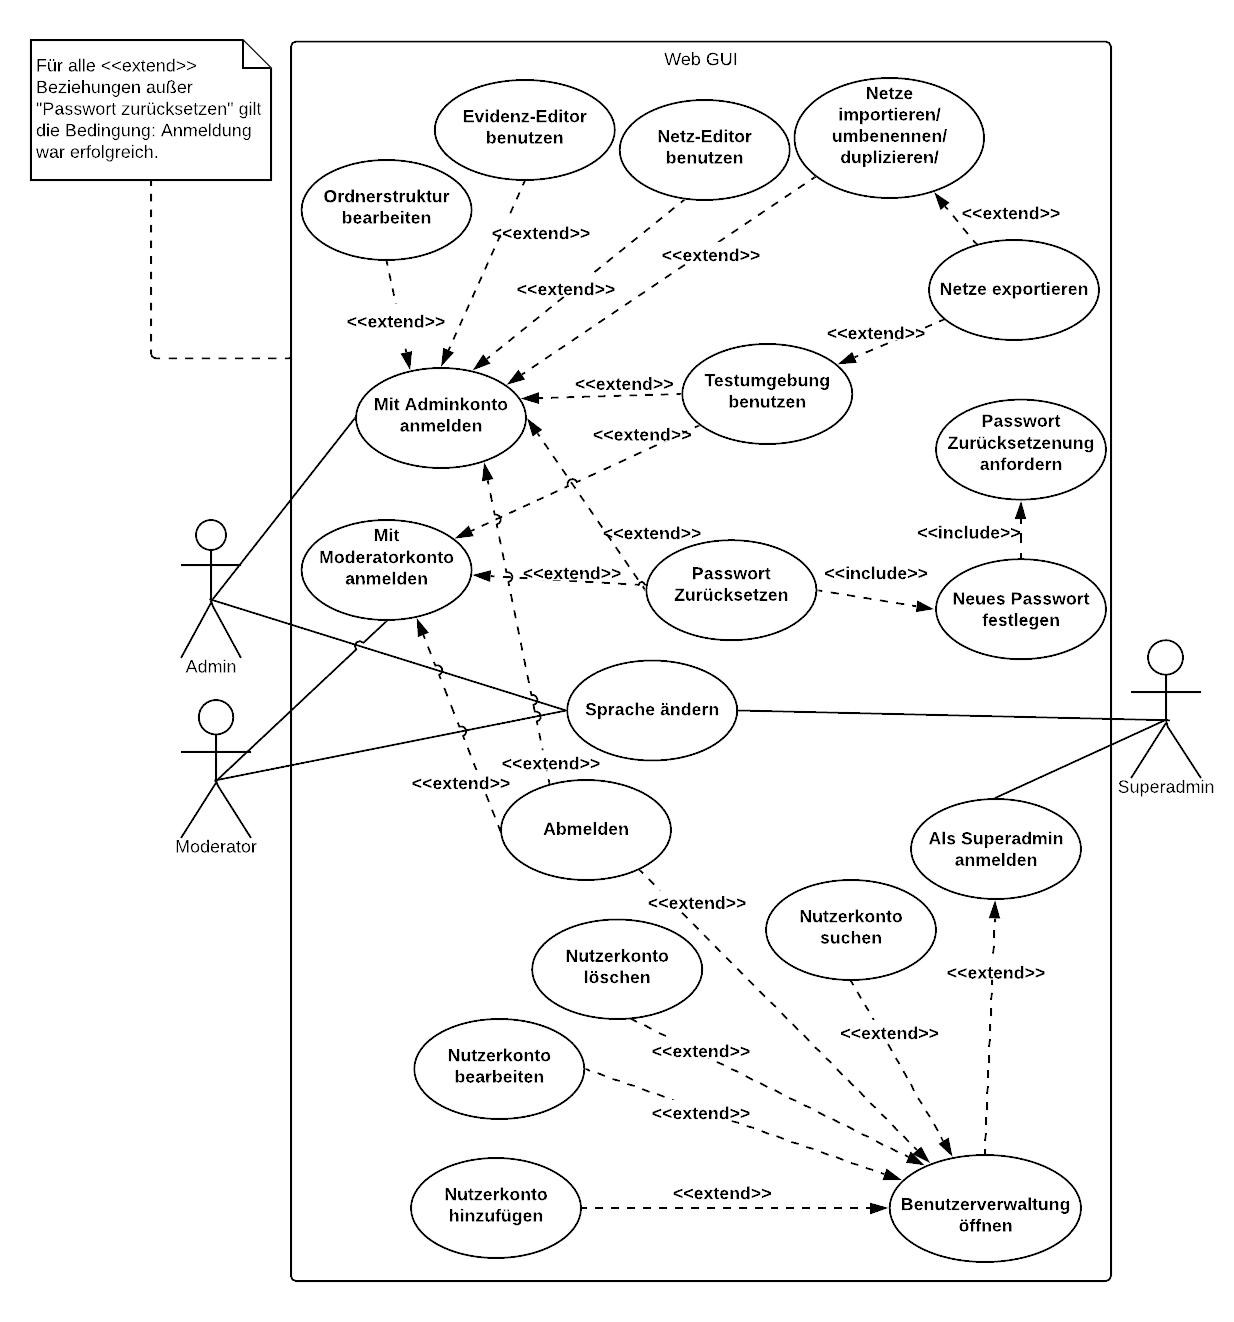
\includegraphics[width=\textwidth,height=\textheight,keepaspectratio]{image/PSEAFv2.png}
   \caption{Anwendungsfalldiagramm GUI}
   \label{fig:af1}
\end{figure}
\pagebreak

\subsection{Anwendungsfälle}

\subsubsection{Superadmin}
Der Superadmin kann sich mit seinen Daten anmelden und somit die Benutzerverwaltung öffnen. Die Benutzerverwaltung verfügt die Option zum Suchen, Hinzufügen, Bearbeiten und zum Löschen von Nutzerkonten. Weiterhin kann sich der Superadmin von der Benutzerverwaltung abmelden. Der Admin kann auch jederzeit die Sprache der GUI ändern. 
\subsubsection{Nutzer}
Ein Nutzer (Admin oder Moderator) kann sich mit seinen Daten anmelden, um Zugriff auf die GUI zu erhalten. Dabei hat der Nutzer die Option sein Passwort zurückzusetzen. Dafür muss der Nutzer eine Passwort Zurücksetzung beantragen und dann ein neues Passwort festlegen. Dann kann sich der Nutzer mit dem neuen Passwort anmelden. Der Nutzer kann jederzeit die Sprache der GUI ändern.

Der angemeldete Nutzer (Admin oder Moderator) kann die Testumgebung benutzen um Netze auszuprobieren. Dort gibt es die Option Netze vom Server lokal herunterzuladen. Letztlich kann sich ein erfolgreich angemeldeter Nutzer von der GUI abmelden.

Ein angemeldeter Admin hat zudem die Optionen den Netz-Editor und den Evidenzen-Editor zu benutzen. Der Admin kann auch noch die Ordnerstruktur bearbeiten und Netze verwalten (importieren, umbenennen und duplizieren). 

\begin{figure}[ht!]
  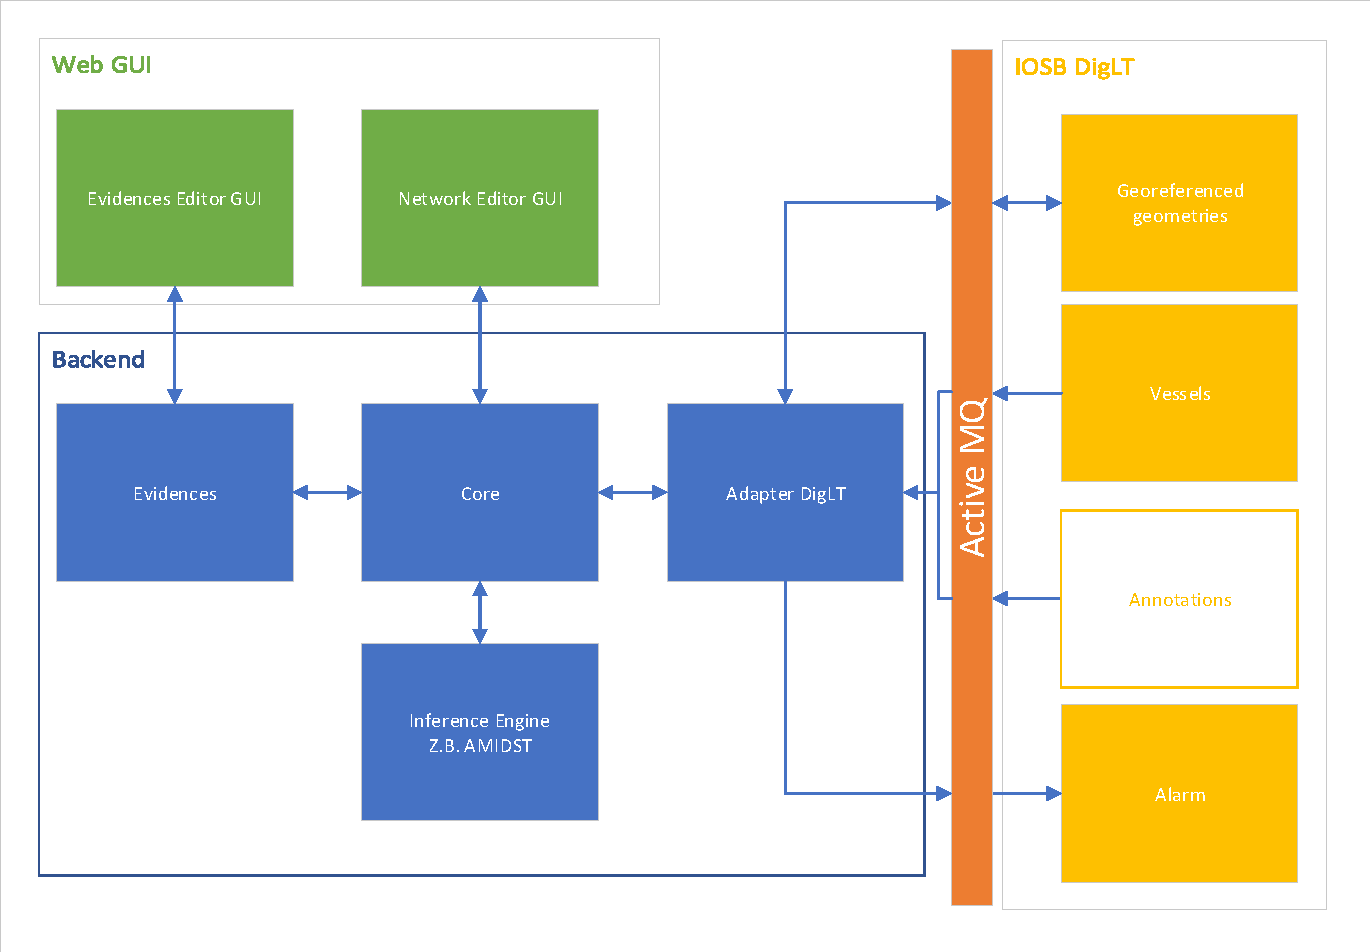
\includegraphics[width=\linewidth]{image/PSE20191028.pdf}
  \caption{Systemmodel}
  \label{fig:Systemmodel}
\end{figure}


\pagebreak
\appendix
\section{GUI-Entwürfe}
\label{section:gui}

\begin{figure}[ht!]
    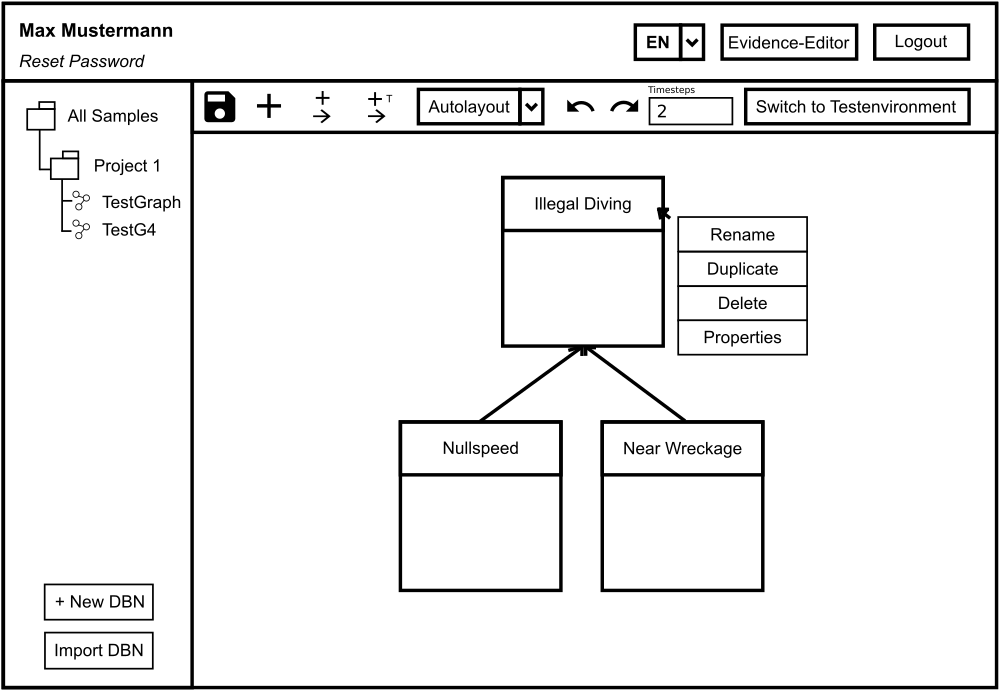
\includegraphics[width=\linewidth]{image/editor.png}
    \caption{Netzeditor mit geöffnetem Rechtsklickmenü des Knotens}
    \label{fig:neteditor}
\end{figure}

\begin{figure}[ht!]
  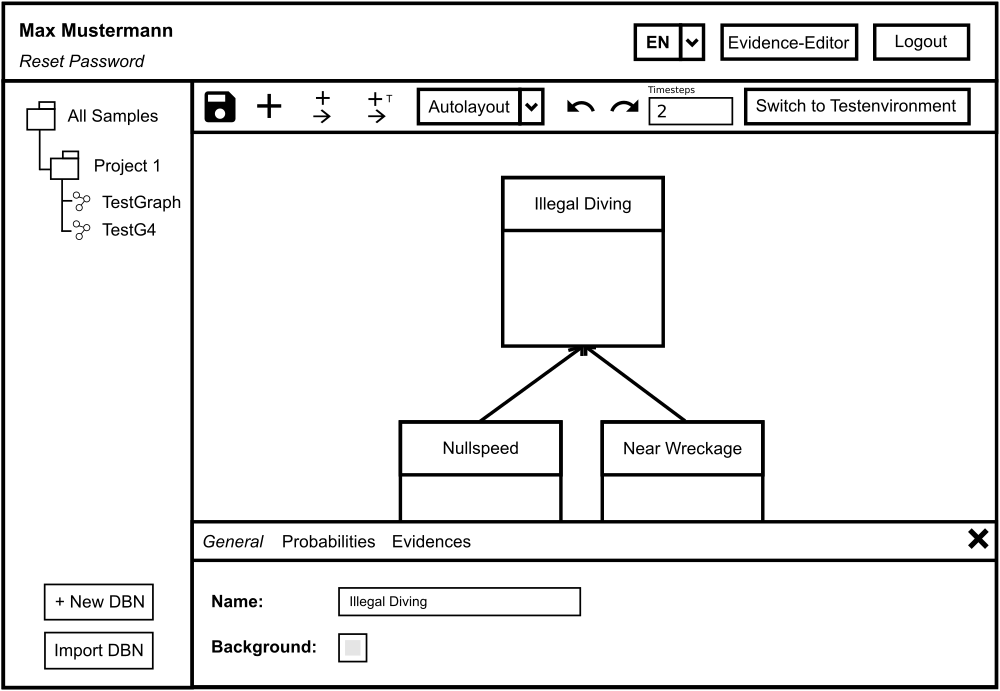
\includegraphics[width=\linewidth]{image/editor_properties.png}
  \caption{Netzeditor mit geöffneten Einstellungen}
  \label{fig:neteditorproperties}
\end{figure}

\begin{figure}[ht!]
  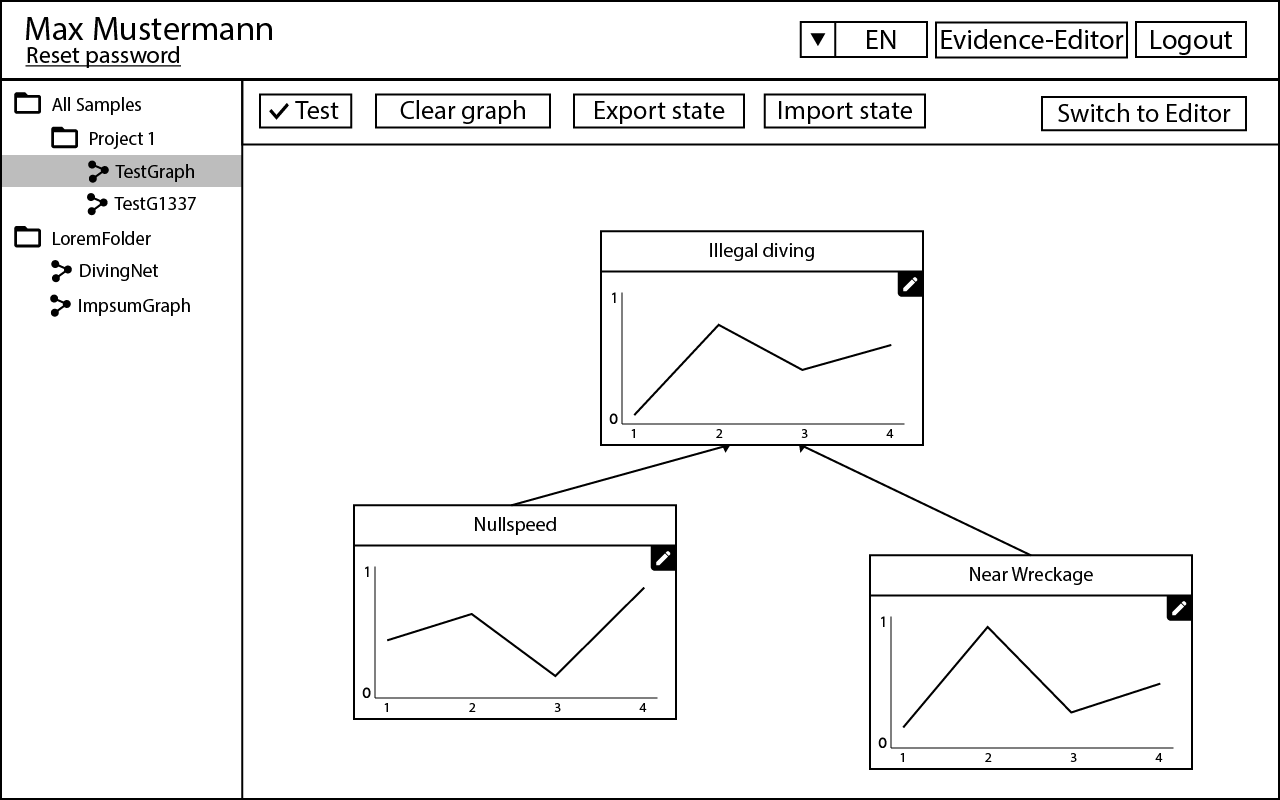
\includegraphics[width=\linewidth]{image/GUI-4.png}
  \caption{Testumgebung für Netze}
  \label{fig:testEdit}
\end{figure}

\begin{figure}[ht!]
  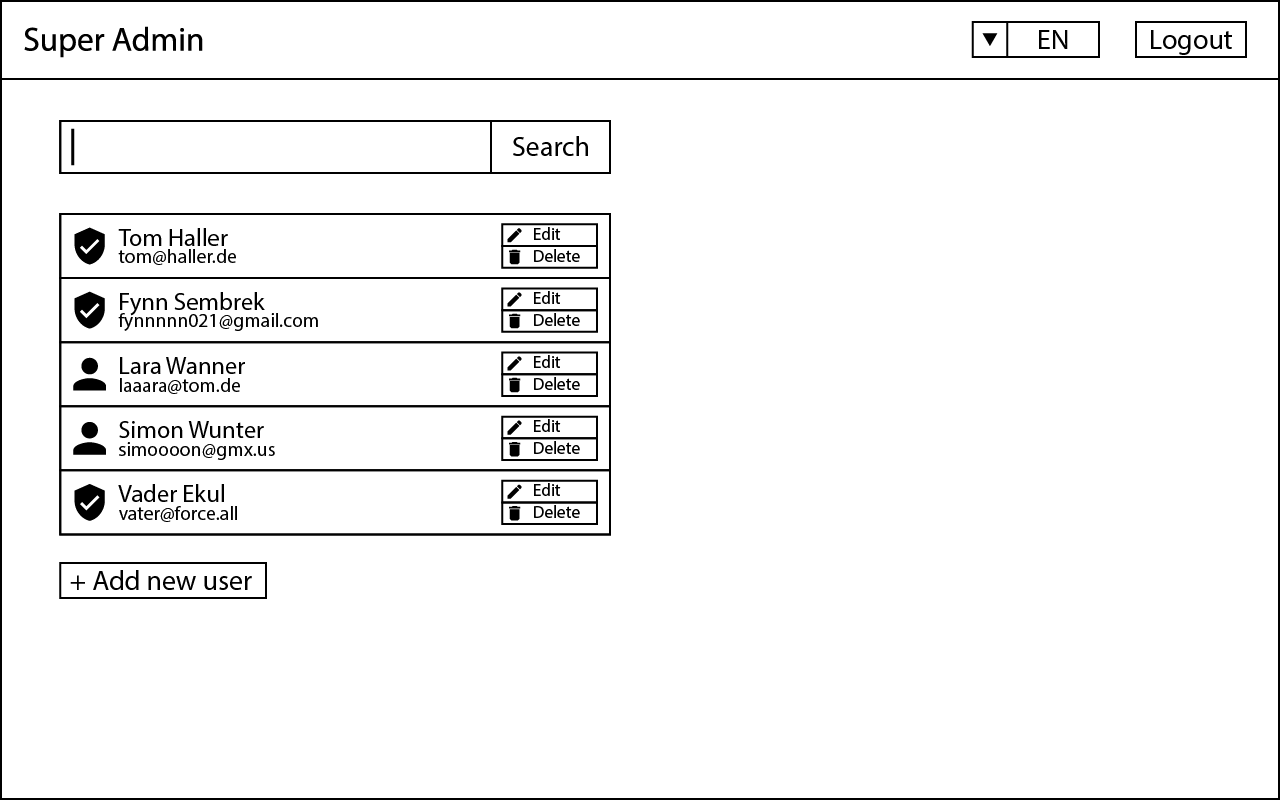
\includegraphics[width=\linewidth]{image/GUI-1.png}
  \caption{Nutzerübersicht des Superadmins}
  \label{fig:saUserview}
\end{figure}

\begin{figure}[ht!]
  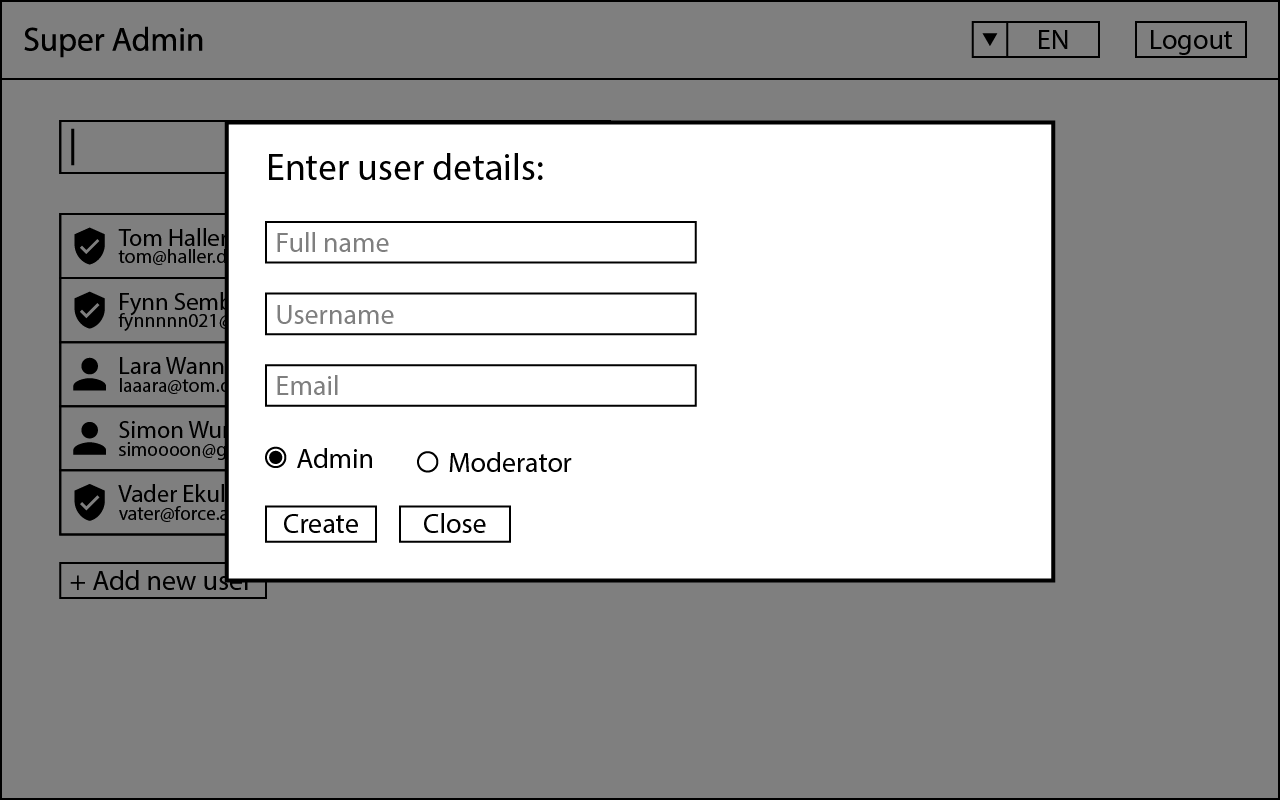
\includegraphics[width=\linewidth]{image/GUI-2.png}
  \caption{Nutzer-Erstellungs Dialog für den Superadmin}
  \label{fig:saCreateUsr}
\end{figure}

\begin{figure}[ht!]
  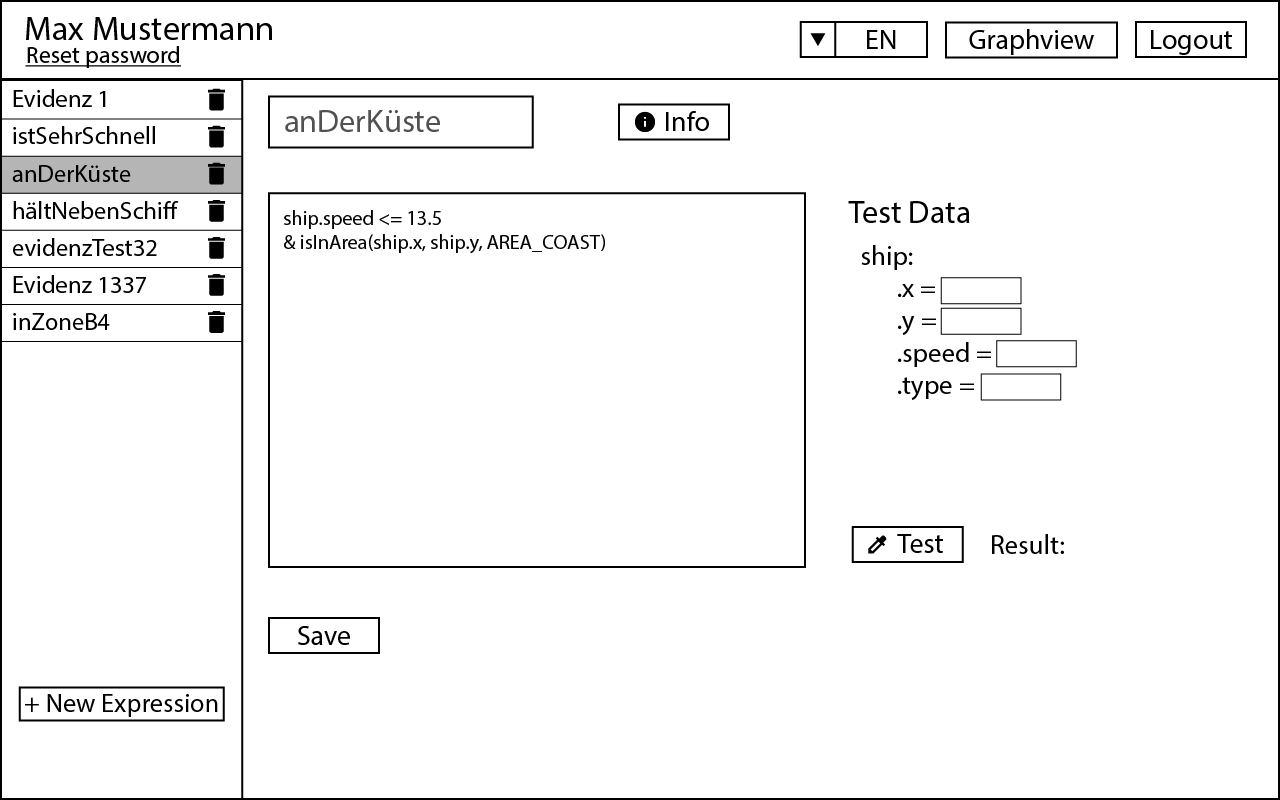
\includegraphics[width=\linewidth]{image/GUI-3.png}
  \caption{Evidez-Formel Editor}
  \label{fig:evdExprEditor}
\end{figure}

% made via https://gomockingbird.com/projects/mnf0cwf/4gXVnC

% \section{Glossar}

\printglossary

\end{document}